%==============================================================================
% Tento soubor použijte jako základ
% This file should be used as a base for the thesis
% Autoři / Authors: 2008 Michal Bidlo, 2022 Jaroslav Dytrych
% Kontakt pro dotazy a připomínky: sablona@fit.vutbr.cz
% Contact for questions and comments: sablona@fit.vutbr.cz
%==============================================================================
% kódování: UTF-8 (zmena prikazem iconv, recode nebo cstocs)
% encoding: UTF-8 (you can change it by command iconv, recode or cstocs)
%------------------------------------------------------------------------------
% zpracování / processing: make, make pdf, make clean
%==============================================================================
% Soubory, které je nutné upravit nebo smazat: / Files which have to be edited or deleted:
%   projekt-20-literatura-bibliography.bib - literatura / bibliography
%   projekt-01-kapitoly-chapters.tex - obsah práce / the thesis content
%   projekt-01-kapitoly-chapters-en.tex - obsah práce v angličtině / the thesis content in English
%   projekt-30-prilohy-appendices.tex - přílohy / appendices
%   projekt-30-prilohy-appendices-en.tex - přílohy v angličtině / appendices in English
%==============================================================================
% \documentclass[]{fitthesis} % bez zadání - pro začátek práce, aby nebyl problém s překladem
% \documentclass[english]{fitthesis} % without assignment - for the work start to avoid compilation problem
% \documentclass[zadani]{fitthesis} % odevzdani do IS VUT a/nebo tisk s barevnými odkazy - odkazy jsou barevné
\documentclass[english,zadani]{fitthesis} % for submission to the IS VUT and/or print with color links - links are color
%\documentclass[zadani,print]{fitthesis} % pro černobílý tisk - odkazy jsou černé
%\documentclass[english,zadani,print]{fitthesis} % for the black and white print - links are black
%\documentclass[zadani,cprint]{fitthesis} % pro barevný tisk - odkazy jsou černé, znak VUT barevný
%\documentclass[english,zadani,cprint]{fitthesis} % for the print - links are black, logo is color
% * Je-li práce psaná v anglickém jazyce, je zapotřebí u třídy použít 
%   parametr english následovně:
%   If thesis is written in English, it is necessary to use 
%   parameter english as follows:
%      \documentclass[english]{fitthesis}
% * Je-li práce psaná ve slovenském jazyce, je zapotřebí u třídy použít 
%   parametr slovak následovně:
%   If the work is written in the Slovak language, it is necessary 
%   to use parameter slovak as follows:
%      \documentclass[slovak]{fitthesis}
% * Je-li práce psaná v anglickém jazyce se slovenským abstraktem apod., 
%   je zapotřebí u třídy použít parametry english a enslovak následovně:
%   If the work is written in English with the Slovak abstract, etc., 
%   it is necessary to use parameters english and enslovak as follows:
%      \documentclass[english,enslovak]{fitthesis}

% Základní balíčky jsou dole v souboru šablony fitthesis.cls
% Basic packages are at the bottom of template file fitthesis.cls
% zde můžeme vložit vlastní balíčky / you can place own packages here


% Pro seznam zkratek lze využít balíček Glossaries - nutno odkomentovat i níže a při kompilaci z konzoly i v Makefile (plnou verzi pro Perl, nebo lite)
% The Glossaries package can be used for the list of abbreviations - it is necessary to uncomment also below. When compiling from the console also in the Makefile (full version for Perl or lite)
%\usepackage{glossaries}
%\usepackage{glossary-superragged}
%\makeglossaries 

% Nastavení cesty k obrázkům
% Setting of a path to the pictures
%\graphicspath{{obrazky-figures/}{./obrazky-figures/}}
%\graphicspath{{obrazky-figures/}{../obrazky-figures/}}

%---rm---------------
\renewcommand{\rmdefault}{lmr}%zavede Latin Modern Roman jako rm / set Latin Modern Roman as rm
%---sf---------------
\renewcommand{\sfdefault}{qhv}%zavede TeX Gyre Heros jako sf
%---tt------------
\renewcommand{\ttdefault}{lmtt}% zavede Latin Modern tt jako tt

% vypne funkci šablony, která automaticky nahrazuje uvozovky,
% aby nebyly prováděny nevhodné náhrady v popisech API apod.
% disables function of the template which replaces quotation marks
% to avoid unnecessary replacements in the API descriptions etc.
\csdoublequotesoff

\usepackage{url}

% =======================================================================
% balíček "hyperref" vytváří klikací odkazy v pdf, pokud tedy použijeme pdflatex
% problém je, že balíček hyperref musí být uveden jako poslední, takže nemůže
% být v šabloně
% "hyperref" package create clickable links in pdf if you are using pdflatex.
% Problem is that this package have to be introduced as the last one so it 
% can not be placed in the template file.
\ifWis
\ifx\pdfoutput\undefined % nejedeme pod pdflatexem / we are not using pdflatex
\else
  \usepackage{color}
  \usepackage[unicode,colorlinks,hyperindex,plainpages=false,pdftex]{hyperref}
  \definecolor{hrcolor-ref}{RGB}{223,52,30}
  \definecolor{hrcolor-cite}{HTML}{2F8F00}
  \definecolor{hrcolor-urls}{HTML}{092EAB}
  \hypersetup{
	linkcolor=hrcolor-ref,
	citecolor=hrcolor-cite,
	filecolor=magenta,
	urlcolor=hrcolor-urls
  }
  \def\pdfBorderAttrs{/Border [0 0 0] }  % bez okrajů kolem odkazů / without margins around links
  \pdfcompresslevel=9
\fi
\else % pro tisk budou odkazy, na které se dá klikat, černé / for the print clickable links will be black
\ifx\pdfoutput\undefined % nejedeme pod pdflatexem / we are not using pdflatex
\else
  \usepackage{color}
  \usepackage[unicode,colorlinks,hyperindex,plainpages=false,pdftex,urlcolor=black,linkcolor=black,citecolor=black]{hyperref}
  \definecolor{links}{rgb}{0,0,0}
  \definecolor{anchors}{rgb}{0,0,0}
  \def\AnchorColor{anchors}
  \def\LinkColor{links}
  \def\pdfBorderAttrs{/Border [0 0 0] } % bez okrajů kolem odkazů / without margins around links
  \pdfcompresslevel=9
\fi
\fi
% Řešení problému, kdy klikací odkazy na obrázky vedou za obrázek
% This solves the problems with links which leads after the picture
\usepackage[all]{hypcap}


% Informace o práci/projektu / Information about the thesis
%---------------------------------------------------------------------------
\projectinfo{
  %Prace / Thesis
  project={DP},            %typ práce BP/SP/DP/DR  / thesis type (SP = term project)
  year={2023},             % rok odevzdání / year of submission
  date=\today,             % datum odevzdání / submission date
  %Nazev prace / thesis title
  title.cs={Tvorba vícejazyčné datové sady pro fact-checking z existujících dat\\pro odpovídání na otázky},  % název práce v češtině či slovenštině (dle zadání) / thesis title in czech language (according to assignment)
  title.en={Designing a Multilingual Fact-Checking\\Dataset from Existing Question-Answering Data}, % název práce v angličtině / thesis title in english
  %title.length={14.5cm}, % nastavení délky bloku s titulkem pro úpravu zalomení řádku (lze definovat zde nebo níže) / setting the length of a block with a thesis title for adjusting a line break (can be defined here or below)
  %sectitle.length={14.5cm}, % nastavení délky bloku s druhým titulkem pro úpravu zalomení řádku (lze definovat zde nebo níže) / setting the length of a block with a second thesis title for adjusting a line break (can be defined here or below)
  %dectitle.length={14.5cm}, % nastavení délky bloku s titulkem nad prohlášením pro úpravu zalomení řádku (lze definovat zde nebo níže) / setting the length of a block with a thesis title above declaration for adjusting a line break (can be defined here or below)
  %Autor / Author
  author.name={Daniel},   % jméno autora / author name
  author.surname={Kamenický},   % příjmení autora / author surname 
  author.title.p={Bc.}, % titul před jménem (nepovinné) / title before the name (optional)
  %author.title.a={Ph.D.}, % titul za jménem (nepovinné) / title after the name (optional)
  %Ustav / Department
  department={UPGM}, % doplňte příslušnou zkratku dle ústavu na zadání: UPSY/UIFS/UITS/UPGM / fill in appropriate abbreviation of the department according to assignment: UPSY/UIFS/UITS/UPGM
  % Školitel / supervisor
  supervisor.name={Martin},   % jméno školitele / supervisor name 
  supervisor.surname={Fajčík},   % příjmení školitele / supervisor surname
  supervisor.title.p={Ing.},   %titul před jménem (nepovinné) / title before the name (optional)
  % supervisor.title.a={Ph.D.},    %titul za jménem (nepovinné) / title after the name (optional)
  % Klíčová slova / keywords
  keywords.cs={Zpracování Přirozeného jazyka, Ověřování Faktů, Získávání Informací, Transformers, mDPR}, % klíčová slova v českém či slovenském jazyce / keywords in czech or slovak language
  keywords.en={Natural Language Processing, Fact-Checking, Information Retrieval, Multilingual, Transformers, mDPR}, % klíčová slova v anglickém jazyce / keywords in english
  %keywords.en={Here, individual keywords separated by commas will be written in English.},
  % Abstrakt / Abstract
  abstract.cs={Tato práce se zabývá nedostatkem vícejazyčných datových sad pro kontrolu faktů, které by obsahovaly důkazy podporující nebo vyvracející fakt. Proto se tato práce zabývá převodem datového souboru pro kontrolu faktů z již existujícího datového souboru otázek a odpovědí. V této práci jsou studovány dva přístupy ke konverzi datové sady. Prvním přístupem je vytvoření datové sady založené na jednojazyčném předem natrénovaném seq-2-seq modelu T5. Model je trénován na anglickém datovém souboru. Vstupy a výstupy jsou překládány do požadovaných jazyků. Druhým přístupem je využití vícejazyčného modelu mT5, který přebírá vstup a generuje výstup v požadovaném jazyce. Pro vícejazyčný model je zapotřebí přeložit trénovací datové sady. Jako hlavní problém této práce se ukázal překlad, který v málo zdrojovém jazyce dosáhl kolem 30\,\% úspěšnosti. Experimenty ukázaly lepší výsledky v tvrzeních generovaných z jednojazyčného modelu s využitím strojového překladu. Na druhou stranu, tvrzení generované z vícejazyčného modelu dosáhly úspěšnosti 73\,\% oproti tvrzením z jednojazyčného modelu s dosaženou úspěšností 88\,\%. Modely byly vyhodnoceny modelem ověřování faktů založeném na TF-IDF. Dosažená přesnost modelu na obou datových sadách se blíží 0,5. Z toho lze usoudit, že výsledné datové sady mohou být náročné pro modely ověřování faktů.}, % abstrakt v českém či slovenském jazyce / abstract in czech or slovak language
  abstract.en={This thesis adresses the lack of multilingual fact-Checking datasets, which contain annotated evidence grounding the supporting or refuting verdict for a fact. Therefore, this work explores the conversion into the fact-checking dataset from an already existing question-answering dataset. In this work, two approaches for converting question-answer pairs into claims are studied. The first approach is to create a dataset based on a monolingual pre-trained seq-2-seq model T5. The model is trained on an English dataset and the inputs and outputs are translated into the desired languages. The second approach is to use the multilingual mT5 model, which can take input and generate output in the desired language. For multilingual model, training datasets need to be translated. The main problem of this work is the machine translation, which achieved around 30\,\% success rate in a \emph{low-resource} languages. The experiments showed better results for claims generated from monolingual model using machine translation. On the other hand, the claims generated from multilingual model achieved a success rate of 73\,\% compared to monolingual model with a success rate of 88\,\%. Finally, to analyze possible biases label specific claim biases, a logistic-regression based TF-IDF classifier is trained. The classifier, that computes the probability of the claim's veracity just from itself achieves accuracy close to  0.5 for both converted datasets. Thus the converted datasets can be challenging for fact-checking models.}, % abstrakt v anglickém jazyce / abstract in english
  %abstract.en={An abstract of the work in English will be written in this paragraph.},
  % Prohlášení (u anglicky psané práce anglicky, u slovensky psané práce slovensky; u projektové praxe lze zakomentovat) / Declaration (for thesis in english should be in english; for project practice can be commented out)
%   declaration={Prohlašuji, že jsem tuto bakalářskou práci vypracoval samostatně pod vedením pana X...
% Další informace mi poskytli...
% Uvedl jsem všechny literární prameny, publikace a další zdroje, ze kterých jsem čerpal.},
  declaration={I hereby declare that this Master's thesis was prepared as an original work by the author under the supervision of Ing. Martin Fajčík.
  I have listed all the literary sources, publications and other sources, which were used during the preparation of this thesis.},
  % Poděkování (nepovinné, nejlépe v jazyce práce; nechcete-li, zakomentujte pro skrytí nadpisu) / Acknowledgement (optional, ideally in the language of the thesis; comment out for hiding including heading)
  acknowledgment={I would like to thank my supervisor Ing. Martin Fajčík for his guidance, enthusiasm, patience and willingness to answer all my questions or help with any issues along the way. Thank You.},
  %acknowledgment={Here it is possible to express thanks to the supervisor and to the people which provided professional help
%(external submitter, consultant, etc.).},
  % Rozšířený abstrakt (cca 3 normostrany) - lze definovat zde nebo níže / Extended abstract (approximately 3 standard pages) - can be defined here or below
  extendedabstract={Vzhledem k tomu, že se nepravdivé informace a falešné zprávy stále šíří po internetu a sociálních sítích, je pro udržení pravdivého digitálního prostředí nezbytná potřeba ověřovacích prostředků. V dnešní digitální době je na internetu dostupné obrovské množství informací a pro jednotlivce může být obtížné rozlišit mezi důvěryhodnými a nedůvěryhodnými zdroji. Ověřování faktů může pomoci identifikovat a opravit chyby, zabránit šíření dezinformací a podpořit důvěru v informacích prezentovaných v textu přirozeným jazykem.
  
Ověřování faktů se týká zjišťování pravdivosti informací, které se nacházejí v textové podobě, ať už na webových stránkách, sociálních médiích, novinách nebo jiných zdrojích. S rozsahem a různorodostí dostupných informací je stále obtížnější rozlišit mezi pravdivými a nepravdivými tvrzeními.

V oblasti zpracování přirozeného jazyka se využívají techniky strojového učení a umělé inteligence ke zpracování a analýze textu. Existují metody automatického ověřování faktů, které se snaží identifikovat a klasifikovat pravdivá, nepravdivá a sporná tvrzení. Tyto metody zahrnují extrakci a porovnání informací z různých zdrojů, analýzu jazyka a kontextu, a také využívají dostupná data a znalosti pro srovnání a validaci tvrzení.

Přestože se technologie zpracování přirozeného jazyka neustále zlepšuje, ověřování faktů je stále náročný úkol. Existují různé výzvy, kterým je třeba čelit, jako jsou rychlost a objem informací, přítomnost zaujatosti a dezinformace, a také složitost samotného jazyka.

Ověřování faktů je zásadní pro důvěryhodnost a spolehlivost informací, které konzumujeme. Správné rozpoznání pravdivých a nepravdivých tvrzení má široké uplatnění, například v novinářství, vědeckém výzkumu, právu, ale také pro obyčejného člověka při orientaci ve světě informací.

Tato práce se zabývá problematikou ověřování faktů v oblasti zpracování přirozeného jazyka. Přesněji v nedostatcích vícejazyčných datových sad, které jsou potřeba k správnému natrénování vícejazyčného modelu. Na základě nejlepšího vědomí autora a získaných znalostí bylo zjištěno, že v dnešní době existuje pouze jedna datová sada X-Fact pro vícejazyčné ověřování faktů. Tato datová sada obsahuje jeden z velkých nedostatků a to chybějicí důkazy podporující nebo vyvracející fakta, které jsou obsaženy v datové sadě. Toto zjištění bylo hlavním motivem pro vytvoření této práce, jelikož je v prácí zastáván názor, který klade důraz pro zakomponování důkazu do datové sady.

To vedlo k myšlence převést existující datové sady otázek a odpovědí do datových sad ověřující fakta. Pokus o konverzi datové sady byl již představen v publikaci FaVIQ. Zdá se, že konverze má slibné výsledky, jelikož dnešní datové sady otázek a odpovědí obsahují vše potřebné k jejich konverzi na datové sady pro kontrolu faktů. Páry otázek a odpovědí převedené na tvrzení s důkazy získanými z modelu získávání informací se ukázaly jako dostatečné pro konverzi do datového souboru pro kontrolu faktů. Datová sada pro kontrolu faktů pak obsahuje všechny požadované části a to zejména důkazy faktů. Celá práce zkoumá rožšiření konverze pro vícejazyčné datové sady.

V této práci jsou navržené dva přítupy pro vytváření vícejazyčné datové sady. Prvním přístupem je natrénování jednojazyčného seq-2-seq modelu T5 na anglické datové sadě. Tento model pak převádí otázky a opovědi z různých jazyků získané z vícejazyčných datových sad otázek a odpovědí. Otázky a odpovědi jsou přeložené pomocí strojového překladu do anglického jazyka a poté předány modelu pro vygenerování požadovaného tvrzení. Tvrzení je poté přeloženo zpátky do požadovaného jazyka. Druhým přístupem je natrénování vícejazyčného modelu, který dokáže převzít vstup a vygenerovat tvrzení již v požadovaném jazyce. Pro natrénování vícejazyčného modelu je zapotřebí přeložení trénovacích datových sad. Tyto dva přístupy jsou poté v práci porovnávány.

Modely byly poté vyhodnoceny na základě správnosti překonvertovaných tvrzení. Výsledky ukázaly, že model T5 dosáhl úspěšnosti 88\,\% oproti modelu vícejazyčného modelu mT5, který dosáhl úspěšnosti 73\,\%. Tyto výsledky musí být podloženy faktem, že využité modely pro strojový překlad dosahovaly poměrně špatných výsledků a to zejména na jazycích s nízkými zdroji (low-resource). Z překorventovaných tvrzeních a ostatních důležitých částí (důkaz, označení pravdivosti) byly vytvořené výsledné datové sady. První datová sada obsahuje tvrzení, které byly překonvertovány modelem T5. Druhá datová sada obsahuje tvrzení, které byly překonvertovány modelem mT5. Datové sady byly poté vyhodnoceny na základě obtížnosti pro model ověřování faktů založeném na TF-IDF. Výsledky ukázaly, že dosažená přesnost modelu na obou datových sadách se blížila hodnotě 0.5. To znamená že úspěšnost modelu ověřování faktů není o nic lepší jak náhodný výběr. Z toho lze usoudit, že výsledné datové sady mohou být náročné pro modely ověřování faktů. Na základě všech informací a výsledků uvedených v této práci je závěrem, že konverze datových sad otázek a odpovědí může být velmi přínosná pro budoucnost vícejazyčných modelů ověřování faktů.},
  % extabstract.odd={true}, % Začít rozšířený abstrakt na liché stránce? / Should extended abstract start on the odd page?
  %faculty={FIT}, % FIT/FEKT/FSI/FA/FCH/FP/FAST/FAVU/USI/DEF
  faculty.cs={Fakulta informačních technologií}, % Fakulta v češtině - pro využití této položky výše zvolte fakultu DEF / Faculty in Czech - for use of this entry select DEF above
  faculty.en={Faculty of Information Technology}, % Fakulta v angličtině - pro využití této položky výše zvolte fakultu DEF / Faculty in English - for use of this entry select DEF above
  department.cs={Ústav matematiky}, % Ústav v češtině - pro využití této položky výše zvolte ústav DEF nebo jej zakomentujte / Department in Czech - for use of this entry select DEF above or comment it out
  department.en={Institute of Mathematics} % Ústav v angličtině - pro využití této položky výše zvolte ústav DEF nebo jej zakomentujte / Department in English - for use of this entry select DEF above or comment it out
}

% Rozšířený abstrakt (cca 3 normostrany) - lze definovat zde nebo výše / Extended abstract (approximately 3 standard pages) - can be defined here or above
%\extendedabstract{Do tohoto odstavce bude zapsán výtah (abstrakt) práce v českém (slovenském) jazyce.}
% Začít rozšířený abstrakt na liché stránce? / Should extended abstract start on the odd page?
%\extabstractodd{true}

% nastavení délky bloku s titulkem pro úpravu zalomení řádku - lze definovat zde nebo výše / setting the length of a block with a thesis title for adjusting a line break - can be defined here or above
%\titlelength{14.5cm}
% nastavení délky bloku s druhým titulkem pro úpravu zalomení řádku - lze definovat zde nebo výše / setting the length of a block with a second thesis title for adjusting a line break - can be defined here or above
%\sectitlelength{14.5cm}
% nastavení délky bloku s titulkem nad prohlášením pro úpravu zalomení řádku - lze definovat zde nebo výše / setting the length of a block with a thesis title above declaration for adjusting a line break - can be defined here or above
%\dectitlelength{14.5cm}

% řeší první/poslední řádek odstavce na předchozí/následující stránce
% solves first/last row of the paragraph on the previous/next page
\clubpenalty=10000
\widowpenalty=10000

% checklist
\newlist{checklist}{itemize}{1}
\setlist[checklist]{label=$\square$}

% Kompilace po částech (rychlejší, ale v náhledu nemusí být vše aktuální)
% Compilation piecewise (faster, but not all parts in preview will be up-to-date)
% Další informace viz / For more information see https://www.overleaf.com/learn/latex/Multi-file_LaTeX_projects
% \usepackage{subfiles}

% Nechcete-li, aby se u oboustranného tisku roztahovaly mezery pro zaplnění stránky, odkomentujte následující řádek / If you do not want enlarged spacing for filling of the pages in case of duplex printing, uncomment the following line
% \raggedbottom

\begin{document}
  % Vysazeni titulnich stran / Typesetting of the title pages
  % ----------------------------------------------
  \maketitle
  % Obsah
  % ----------------------------------------------
  \setlength{\parskip}{0pt}

  {\hypersetup{hidelinks}\tableofcontents}
  
  % Seznam obrazku a tabulek (pokud prace obsahuje velke mnozstvi obrazku, tak se to hodi)
  % List of figures and list of tables (if the thesis contains a lot of pictures, it is good)
  % \ifczech
  %   \renewcommand\listfigurename{Seznam obrázků}
  % \fi
  % \ifslovak
  %   \renewcommand\listfigurename{Zoznam obrázkov}
  % \fi
  % {\hypersetup{hidelinks}\listoffigures}
  
  % \ifczech
  %   \renewcommand\listtablename{Seznam tabulek}
  % \fi
  % \ifslovak
  %   \renewcommand\listtablename{Zoznam tabuliek}
  % \fi
  % {\hypersetup{hidelinks}\listoftables}

  % Seznam zkratek / List of abbreviations
  %\ifczech
  %  \renewcommand*\glossaryname{Seznam zkratek}%
  %  \renewcommand*\entryname{Zkratka}
  %  \renewcommand*\descriptionname{Význam}
  %\fi
  %\ifslovak
  %  \renewcommand*\glossaryname{Zoznam skratiek}%
  %  \renewcommand*\entryname{Skratka}
  %  \renewcommand*\descriptionname{Význam}
  %\fi
  %\ifenglish
  %  \renewcommand*\glossaryname{List of abbreviations}%
  %  \renewcommand*\entryname{Abbreviation}
  %  \renewcommand*\descriptionname{Meaning}
  %\fi
  % Definice zkratek - z textu se odkazují např. \Gls{TF–IDF}
  % Definition of abbreviations - referred from the text e.g. \Gls{TF–IDF}
  %\newglossaryentry{TF–IDF}
  %{
  %  name={TF–IDF},
  %  description={Term Frequency-Inverse Document Frequency}
  %}
  % 
  %\setglossarystyle{superragged}
  %\printglossaries


  \ifODSAZ
    \setlength{\parskip}{0.5\bigskipamount}
  \else
    \setlength{\parskip}{0pt}
  \fi

  % vynechani stranky v oboustrannem rezimu
  % Skip the page in the two-sided mode
  \iftwoside
    \cleardoublepage
  \fi

  % Text prace / Thesis text
  % ----------------------------------------------
  \ifenglish
    \chapter{Introduction}
As false information and fake news continue propagating throughout the internet and social networks, the need for fact-checking operations becomes necessary in order to maintain a truthful digital environment. In today's digital age, there is a vast amount of information available online, and it can be difficult for individuals to distinguish between credible sources and unreliable sources. Fact-checking can help to identify and correct errors, prevent the spread of misinformation, and promote trust in the information presented in natural language text. Additionally, in certain fields like journalism, fact-checking is a crucial step to ensure the credibility of the news and protect the public from being misinformed.

From a social and psychological perspective, humans have been proven irrational~\cite{misinformation} and vulnerable when differentiating between real and fake news. In other words, fake news can gain broad public trust relatively easier than truthful news because individuals tend to trust fake news after constant exposure, if it confirms their pre-existing beliefs, or simply due to the obligation of participating socially and proving a social identity.

Based on these findings, efforts are being made to come up with a solution that can distinguish between real and fake news. Fact verification efforts are divided into two distinct approaches, namely manual and automated fact-checking. Manual fact-checking is time consuming and not a sustainable long-term solution like the manual solutions of PolitiFact.com~\footnote{\url{https://www.politifact.com}}, FactCheck.org~\footnote{\url{https://www.factcheck.org}}, FEVER~\cite{fever}, X-Fact~\cite{x-fact} and many others~\cite{fakenewsnet}\cite{liar}\cite{covert}. The amount of disinformation increases over time and the people verifying the facts cannot keep up with the increase in disinformation. On the other hand manual fact-checking is considered to be the most reliable method of verifying the accuracy of information. The other approach is automated fact-checking that has the advantage of being able to perform verification quickly and on a large scale. Automated fact-checking systems can analyze large amounts of text and identify potential errors or inaccuracies much faster than a human fact-checker could. However, there are also some limitations to automated fact-checking. One of the main limitations is that automated fact-checking systems rely on pre-existing knowledge and data, which can be incomplete or out of date. Additionally, automated fact-checking systems may not be able to understand the nuances and context of natural language text, which can lead to false positives or negatives. 

Another major disadvantage is that information can spread beyond the boundaries of language in which it was created. Nowadays, there are several fact-checking models that are based on the English language~\cite{faviq}\cite{fever}\cite{covert}. To verify a fact from another language, a translation is needed, but as the results of this work showed, the translation may not always be correct or not everything can be translated. The problem is all the more obvious for \emph{low-resource} languages. These language can have relatively small vocabulary, limited training data or they exhibit complex grammar, sentence structures, and rich morphology. Therefore there is an effort to create a multilingual model for verifying facts. However, quality data is required to train a multilingual model. Based on the author's best knowledge, one multilingual dataset named X-Fact~\cite{x-fact} was found, which is intended for training and validating a multilingual model, but the individual samples of the dataset lack evidence where the confirmation or refutation of the fact occurred.

This leads to an idea to convert existing question-answer datasets to fact-checking datasets. The first attempt to convert dataset was introduced in paper~\cite{faviq}. The conversion seems to has a promising results as today's question-answer datasets contain everything we need for converting them into fact-checking datasets. It is shown that question-answer pairs converted into the claim with the evidence retrieved from information retrival model are sufficient for the conversion into the fact-checking dataset. A fact-checking dataset then contains all the required parts. Especially evidence, which is considered as the main deficiency in current state-of-the-art and also the research subject of this work.

The rest of the thesis is organised as follows. Chapter~\ref{c2} introduces the basics of all the topics related to and essential to this thesis. The datasets that are considered to be related to this thesis and all the information taken from it's knowledge are described in Chapter~\ref{c3}. Subsequently, the information retrieval models are described in Chapter~\ref{c4}. Chapter~\ref{c5} presents all the proposed systems for the conversion of dataset. The experimental setup with all the metrics used in this thesis is then described in Chapter~\ref{c6}. The experimental evaluation of the converted datasets and other experiments performed within this thesis are discussed in Chapter~\ref{c7}. Finally, the thesis is concluded in Chapter~\ref{c8}.

% ################################################################################################################################################################################
% ################################################################################################################################################################################

\chapter{Preliminaries}\label{c2}
Nowadays, systems are based on existing pre-trained models. Most of the models benefit from prior information that has been developed in the past and try to adapt it for a specific use case. One of the basic qualities required to create something new and beneficial to society is to understand the work that has already been published and be able to apply and possibly modify it to achieve better results.

Several new papers were published, such as the BERT model~\cite{bert}, the T5 model\cite{T5} or the GPT model~\cite{gpt}, which are based on the knowledge gained from the paper discussing transformer~\cite{transformer}. Nowadays, there are publications of models such as~\cite{gpt4} that are still being experimented with. There is still an ongoing effort to find out the limits of the models.

One of the model is the Recurrent Neural Network~\cite{rnn}\cite{elman}. The architecture of RNN is a variation of a basic neural network. RNNs are good for processing sequential data such as natural language processing and audio recognition. But there is one major issue that the RNNs suffer from short-term-memory problems. One of the mostly known issue is the vanishing gradient problem. This is the main problem during the training as the gradients for the weights at each layer are computed via the Chain Rule, their gradient values will exponentially shrink as it propagates through each time step, eventually “vanishing”.

Long Short-Term Memory~\cite{LSTM} (LSTM) and Gated Recurrent Unit~\cite{GRU} (GRU) were proposed to mitigate the vanishing gradient problem. LSTMs use a memory cell that can store information over long periods of time and gating mechanisms that allow them to selectively forget or remember information. GRUs are similar to LSTMs, but they have fewer gating mechanisms and are computationally less expensive.

However RNN, LSTM, and GRU are all types of recurrent neural networks that are designed to work with sequential data, such as natural language text. They are all based on the idea of having a "memory" that allows the network to keep track of previous inputs, enabling the network to model sequential dependencies in the data. Additionally, all three architectures involve passing information between units of the network in a recurrent fashion. This means that the output of a unit can serve as input to another unit in the network, allowing information to flow backwards and forwards in the network.

Thus, even though the vanishing gradient problem has been mitigated, there is still the problem that RNN type models are very slow to train, so much so that truncated back-propagation~\cite{back-propagation} is used to update the parameters. 
% ################################################################################################################################################################################

\section{Transformer} \label{transformer}
Since RNN-based models use sequential data flow, they cannot be parallelized as well as the other type of neural networks called transformer~\cite{transformer}. Transformers are a type of neural network architecture that have revolutionized natural language processing once again. The transformer architecture utilizes a self-attention mechanism, which allows the model to attend to different parts of the input sequence during training.

This self-attention mechanism is able to learn non-trivial alignments between words in the input sequence, which helps the model to better understand the relationships between words in a sentence. This is in contrast to previous approaches such as recurrent neural networks, which process the input sequence one word at a time and have difficulty capturing long-term dependencies. Transformers replaced RNNs in many areas, such as language translation, text classification, question answering, and became new state-of-the-art architecture for language modeling~\cite{transformers_vs_rnn}. 

\subsection{Model architecture}
The network employs an encoder-decoder architecture much like RNNs shown in figure~\ref{fig:transformer}. Only some parts of the architecture are described in this paper. A more precise and complete description of all parts can be found in the publication~\cite{transformer}. The difference is that the input sequence can be passed in parallel compared to RNNs which need to take the input sequence word by word because of the hidden state dependencies. The input sentence is passed to the encoder that generates the input embeddings simultaneously for each word. The decoder then generates an output sequence of symbols. At each step, the model is auto-regressive and consumes the previously generated symbols as the next input when generating the next step.

\begin{figure}[H]
    \centering
    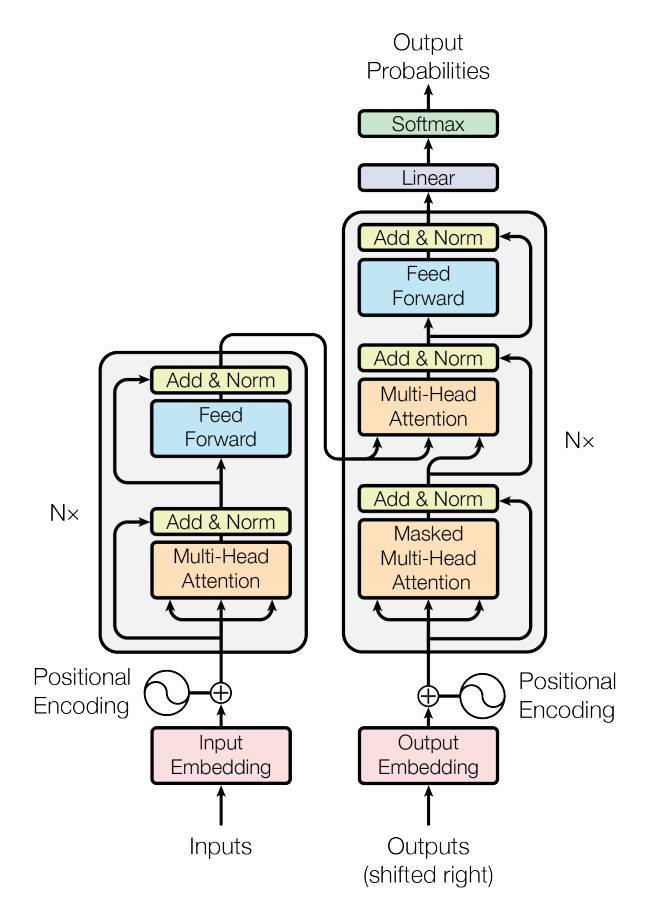
\includegraphics[scale=0.4]{figures/transformer_architecture.jpg}
    \caption{Encoder-Decoder structure of the transformer architecture~\cite{transformer}.}
    \label{fig:transformer}
\end{figure}

\subsubsection*{Scaled Dot-Product Attention}
Scaled Dot-Product Attention is a key component of the self-attention mechanism used in transformers for natural language processing. It involves computing the dot product between a query vector and a set of key vectors, and then using the resulting scores to weight the corresponding value vectors.

Query vector, key vector, and value vector are components of the attention mechanism. In the attention mechanism, the input sequence is mapped into these three vectors using learned linear projections. The query vector is used to attend to specific parts of the input sequence by computing the similarity between the query vector and each key vector. The similarity scores are then used to weight the corresponding value vectors, which are summed up to produce the attended output.

To obtain the query, key, and value vectors, three weight matrices, $\boldsymbol{W}_q$, $\boldsymbol{W}_k$, and $\boldsymbol{W}_v$, are multiplied with the input sequence, and they project the input sequence into the query vector, key vector, and value vector, respectively:

\begin{equation}
    \boldsymbol{Q} = \boldsymbol{XW}_q, \boldsymbol{K} = \boldsymbol{XW}_k, \boldsymbol{V} = \boldsymbol{XW}_v.
\end{equation}

where $\boldsymbol{X}$ is the input sequence, each weight matrix is learned during training to optimize the performance of the model, and the size of the weight matrices depends on the desired dimensionality of the query, key, and value vectors.

Each of the vectors extracts different components of the input token. Thus, for each input token $x_i$, the query vector $q_i$, the key $k_i$ and the value $v_i$ are extracted, where $i$ represents the index of the token in the input sequence. The computation is processed simultaneously. Matrices $\boldsymbol{Q}$, $\boldsymbol{K}$, and $\boldsymbol{V}$ are then used to compute the attention matrix for each word using formula:
\begin{equation}
    \text{Attention}(\boldsymbol{Q},\boldsymbol{K},\boldsymbol{V}) = \text{softmax}(\frac{\boldsymbol{QK}^T}{\sqrt{d_k}})\boldsymbol{V}
\end{equation}
\noindent The computation of the attention function on the set of queries is performed simultaneously, packed in the matrix $\boldsymbol{W}_q$ and keys and values are also packed into matrices $\boldsymbol{W}_k$ and $\boldsymbol{W}_v$. 
Scaled Dot-Product Attention allows the model attend to different parts of the input sequence based on the query, capturing complex dependencies between tokens in the sequence.

\subsubsection*{Multi-Head Attention}
Multi-Head Attention is an extension of the Scaled Dot-Product Attention mechanism used in transformers for natural language processing. It allows the model to attend to different parts of the input sequence simultaneously, by computing multiple attention functions in parallel. The input query vector $\boldsymbol{Q} \in \mathbb{R}^{d_q}$, key vector $\boldsymbol{K} \in \mathbb{R}^{d_k}$, and value vectors $\boldsymbol{V} \in \mathbb{R}^{d_v}$ are linearly projected $h$ times with different learned linear projections $\boldsymbol{W}_q^i \in \mathbb{R}^{d_q \times d_h}$, $\boldsymbol{W}_k^i \in \mathbb{R}^{d_k \times d_h}$, and $\boldsymbol{W}_v^i \in \mathbb{R}^{d_v \times d_h}$ respectively, as each of these linear projections are learned independently.

Here, $d_q$, $d_k$, and $d_v$ represent the dimensions of the query vector, key vector, and value vectors, respectively. $h$ represents the number of times these vectors are linearly projected, and $i$ represents the index of each projection. $\boldsymbol{W}_q^i$, $\boldsymbol{W}_k^i$, and $\boldsymbol{W}_v^i$ represent the learned linear projections for query, key, and value vectors, respectively. The outputs from each of the attention head is then concatenated and once again projected, resulting in the final values, as depicted in Figure~\ref{fig:multi_head}.

\begin{figure}[H]
    \centering
    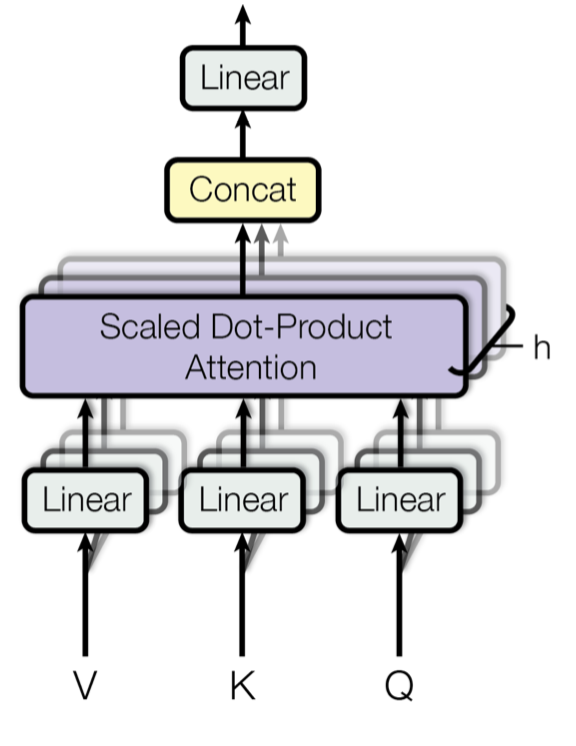
\includegraphics[scale=0.3]{figures/multi-head-attention.png}
    \caption{Multi-Head Attention layer}
    \label{fig:multi_head}
\end{figure}

Multi-head attention allows the model to jointly attend to information from different representation subspaces at different positions. 

\section{BERT}
BERT~\cite{bert} stands for Bidirectional Encoder Representations from Transformers and it is a~model that is pre-trained on unsupervised tasks using large amount of data. The pre-trained BERT model can be fine-tuned with just one additional output layer, without needing to retrain the entire model, for a wide range of tasks, such as question-answering and Natural Language Inference.
\subsection*{Architecture}
BERT’s model architecture consists of a multi-layer bidirectional Transformer encoder based on the original implementation of transformer~\cite{transformer}. The architecture is identical with the transformer model section~\ref{transformer}.

BERT model was published in two different model sizes: $\text{BERT}_{\textsc{BASE}}$ model consists of 12 layers (i.e., transformer blocks), with the hidden size of 768 and 12 self-attention heads resulting in a total of 110M parameters and $\text{BERT}_{\textsc{LARGE}}$ model consists of 24 layers (i.e., transformer blocks) with the hidden size of 1024 and 16 self-attention heads resulting in a total of 340M parameters.

\subsection*{Training}
The model was pre-trained on two unsupervised tasks namely Masked Language Modeling and Next Sentence Prediction which will be explained below. For fine-tuning, the BERT model is first initialized with the pre-trained parameters, and all of the parameters are fine-tuned using labeled data from the downstream tasks. Each downstream task has separate fine-tuned models, even though they are initialized with the same pre-trained parameters. The process of the fine-tuning and the pre-training is shown in figure~\ref{fig:bert}, where \texttt{[CLS]} is a special classification token that is the first token of every sentence, \texttt{[SEP]} is token for differentiation of the sentence pairs, input embeddings are denoted as \emph{E}, the final hidden vector for special token \texttt{[CLS]} is denoted as \emph{C} and the final hidden vector for the $i^{th}$ input token is denoted as $T_i$. The final hidden vector refers to the output of the BERT model for a given input sequence. Specifically, BERT consists of a stack of transformer layers, where each layer takes in an input sequence and generates a new sequence of hidden states. The final hidden vector is the hidden state corresponding to the special \texttt{[CLS]} token that is added at the beginning of the input sequence.

\begin{figure}[h]
    \centering
    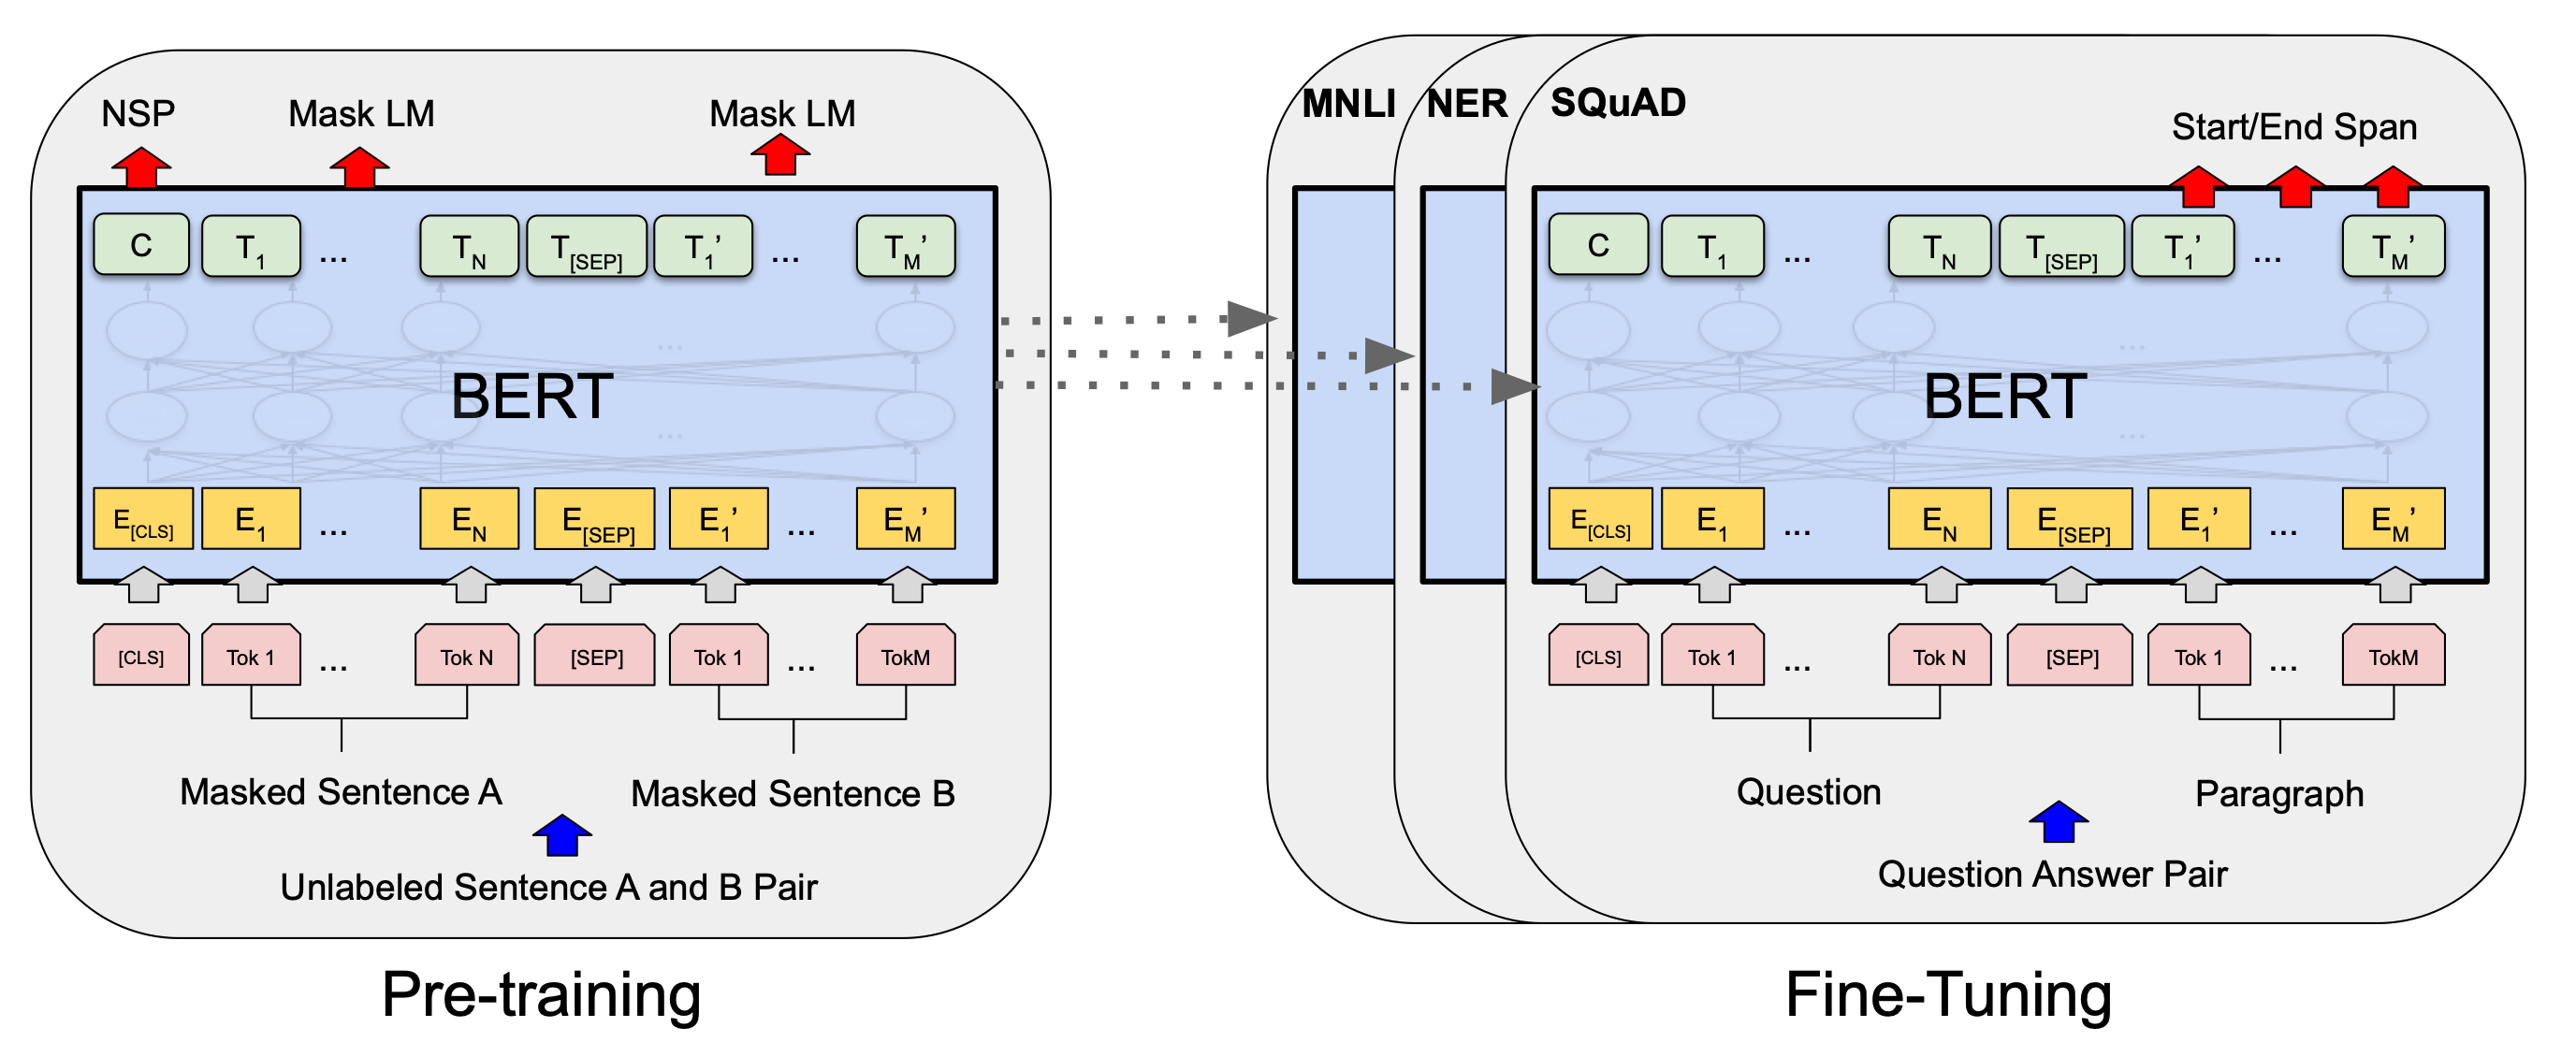
\includegraphics[scale=0.15]{figures/bert.png}
    \caption{The question-answering example of overall pre-training and fine-tuning procedures for BERT~\cite{bert}. For different tasks (NER~\cite{ner}, MNLI~\cite{mnli} and QA) the same initialization of the pre-trained model parameters is used.}
    \label{fig:bert}
\end{figure}

\subsubsection*{Masked Language Modeling (MLM)}\label{MLM}
Masked Language Modeling (MLM) is a task in natural language processing that involves masking some words in a sentence and then predicting the masked words based on the context.

The BERT model was pre-trained by masking 15\,\% of the input tokens and then predicting these masked tokens. In the publication~\cite{bert}, they refer to this procedure as a “masked Language Modeling” (MLM), although it is often referred to as a Cloze task in the literature~\cite{cloze}.

However, since the \texttt{[MASK]} token does not appear during fine-tuning, this leads to mismatch in pre-training and fine-tuning. To mitigate this, masked tokens are not always masked by the \texttt{[MASK]} token, but only in 80\,\% of the time. In the remaining 10\,\% of the time, the masked token is replaced by a random token, and in the last 10\,\% of the time the masked token is not changed. 

\subsubsection*{Next Sentence Prediction (NSP)}
For some important tasks like Question-Answering, it is not enough to train only on language modeling, but it also rely on understanding the relationship between two sentences, that is not directly captured by MLM. Therefore, the model is trained on pairs of sentences to predict whether the next sentence is following the first sentence in the original text or not. This is done by choosing sentence \texttt{A} and \texttt{B} in the way that in the 50\,\% of the time the sentence \texttt{B} is the actual next sentence that follows \texttt{A} and 50\,\% of the time it is a random sentence from the corpus. The sentences are separated with the special token \texttt{[CLS]} and the result of the next sentence prediction is then denoted as $C$ shown in figure~\ref{fig:bert}. However, this objective was shown to be redundant since RoBERTa paper~\cite{roberta}.

% ################################################################################################################################################################################

\section{Text-to-text transfer transformer}\label{T5}
The Text-to-Text Transfer Transformer~\cite{T5} (T5) is a language model that is based on the transformer architecture and is trained in a text-to-text framework, meaning that it is trained to generate text outputs from text inputs. T5 is trained on a diverse set of tasks, including machine translation, summarization, question answering, and text classification, among others. This makes it a highly versatile language model that can be fine-tuned for a wide range of downstream tasks with relatively little additional training data.

\subsection*{Architecture}
The T5 model is based on the Transformer encoder-decoder architecture~\cite{transformer} as it has been found to perform well in both generative and classification tasks. The encoder and decoder are each designed to be similar in size, specifically, both consist of 12 blocks, each block comprising self-attention, optional encoder-decoder attention, and a feed-forward network~\cite{feed-forward}. The ``key'' and ``value'' matrices of all attention mechanisms have an inner dimensionality of $d_{kv}$ = 64 and all attention mechanisms have 12 heads. The feed-forward networks in each block consist of a dense layer with an output dimensionality of $d_{\text{ff}}$ = 3072 followed by a ReLU~\cite{relu} nonlinearity and another dense layer. All other sub-layers and embeddings have a dimensionality of $d_{\text{model}}$ = 768. The model contains about 220 million parameters and uses a dropout probability of 0.1 for regularization. A dropout probability of 0.1 is applied everywhere dropout is used in the model. 

Dropout probability is a regularization technique used to prevent overfitting in neural networks. During training, a certain proportion of randomly selected neurons in a layer are dropped out, meaning their outputs are set to zero. 

\subsection*{Training data}
To create a dataset, Common Crawl was used as a source of text. Due to the scraped text data a significant portion of it is not natural language. It consists of gibberish, duplicate text, menus, error messages, and other non-useful content. To clean up Common Crawl’s web extracted text, several heuristics were employed. These include retaining lines that end in a terminal punctuation mark, discarding pages with fewer than five sentences, removing any page containing a word on the ``List of Dirty, Naughty, Obscene or Otherwise Bad Words''\footnote{\url{https://github.com/LDNOOBW/List-of-Dirty-Naughty-Obscene-and-Otherwise-Bad-Words}}, removing any line with the word Javascript, among others. The dataset was then posprocessed with use of \texttt{langdetect}\footnote{\url{https://pypi.org/project/langdetect/}} to filtered out any pages that were not classified as English with a probability of at least 0.99.

To assemble the base data set, the web extracted text from April 2019 was downloaded, and the aforementioned filtering was applied. This produced a collection of text known as the ``Colossal Clean Crawled Corpus'' (C4).

\subsection*{Pre-training tasks}\label{t5_pretraining}
An objective that does not require labels but teaches the model generalizable knowledge is necessary for leveraging unlabeled data to pre-train the model. Inspired by BERT’s “Masked Language Modeling” objective (described in section~\ref{MLM}) and the “word dropout” regularization technique~\cite{regularization}, an objective is designed that randomly samples and then drops out 15\,\% of tokens in the input sequence. All consecutive spans of dropped-out tokens are replaced by a single sentinel token. A token ID that is unique to the sequence is assigned to each sentinel token. The sentinel IDs are special tokens which are added to the vocabulary and do not correspond to any wordpiece. The target then corresponds to all of the dropped-out spans of tokens, delimited by the same sentinel tokens used in the input sequence plus a final sentinel token to mark the end of the target sequence.

\begin{figure}[H]
    \centering
    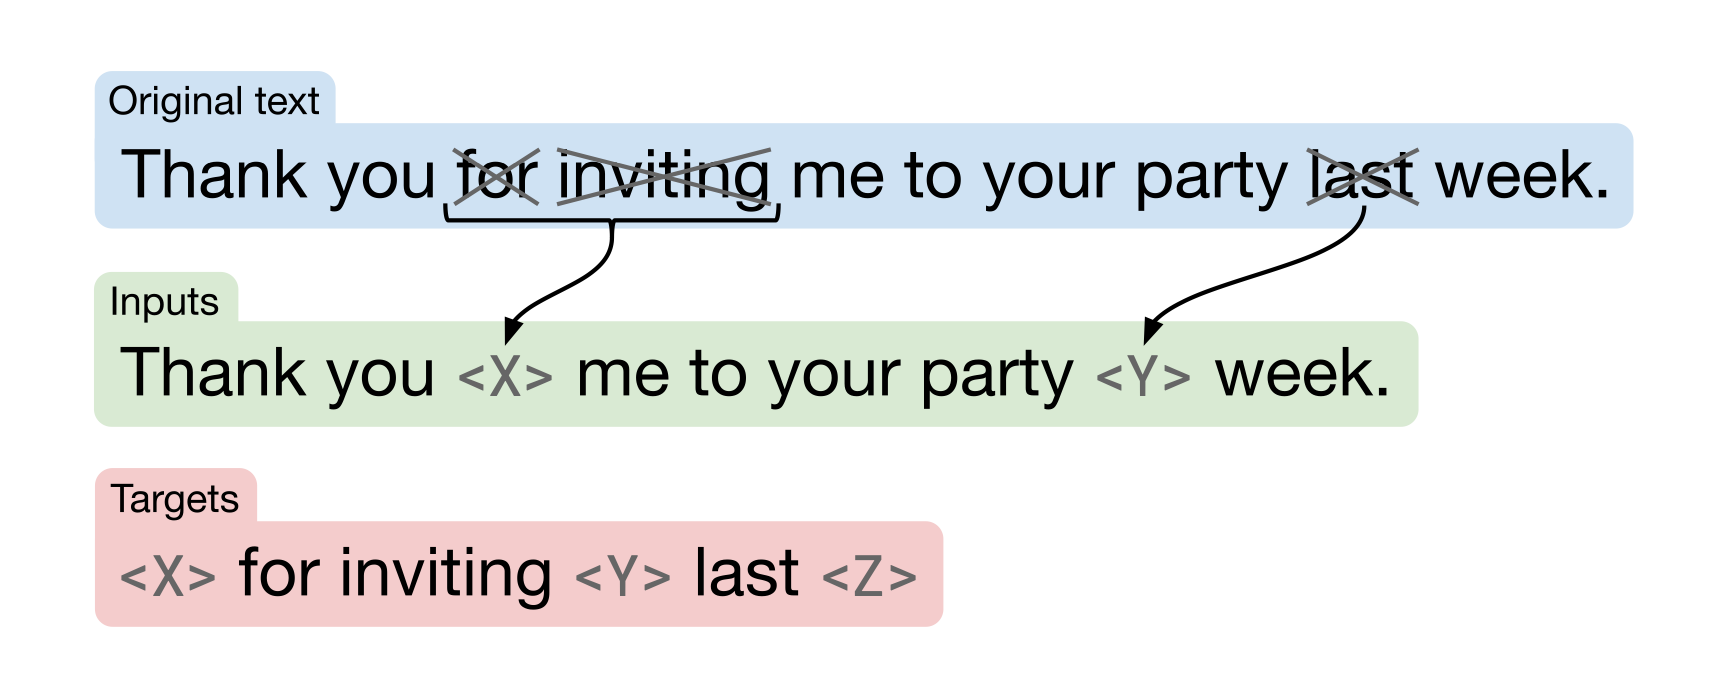
\includegraphics[scale=0.2]{figures/t5_pretraining.png}
    \caption{Schematic of the objective for pre-training.}
    \label{fig:t5_pretraining}
\end{figure}

\subsection*{Downstream tasks}
Downstream tasks were chosen to measure general language learning abilities. Therefore diverse set of benchmarks were used including machine translation, question answering, abstractive summarization, and text classification. Specifically the performance of the model was measured on the GLUE~\cite{glue} and SuperGLUE~\cite{superglue} text classification, CNN/Daily Mail abstractive summarization~\cite{daily_mail}, SQuAD question answering~\cite{squad} and WMT English to German, French and Romanian translation~\cite{wmt}.

\subsection*{Input and output format}
A "text-to-text" format is used to cast all the tasks considered for training a single model in order to provide a consistent training objective for both pre-training and fine-tuning. In this format, the model is given some text as context or conditioning and is then required to produce some output text. The maximum likelihood objective is used to train the model, using ``teacher forcing''~\cite{teacher_forcing} regardless of the task. To indicate which task the model should perform, a task-specific prefix is added to the original input sequence before it is fed to the model. The example of the input sequence is shown in section~\ref{t5_proposed}.

\subsection*{Training}
All the tasks were formulated as text-to-text tasks. This allowed always to the training use standard maximum likelihood and a cross-entropy loss. For optimization the AdaFactor was used. At test time the greedy decoding was used (i.e. choosing the highest-probability logit at every timestep).

The model was pre-trained on the C4 dataset for 524,288 steps. The maximum sequence length was set to 512 and the batch size was set to 128 sequences. The "inverse square root" was used as the learning rate schedule: $1/\sqrt{\text{max}(n,k)}$, where n is the current training iteration and k is the number of warm-up steps. The warm-up steps were set to $10^4$. This set a constant learning rate of 0.01 for the first $10^4$ steps and then exponentially decreased the learning rate until pre-training was over.

The model was then fine-tuned on all the downstream tasks for 262,144 steps. This value was chosen as a trade-off between the high-resource tasks, which benefit from additional fine-tuning, and low-resource task, which overfit quickly. The maximum sequence length and batch size were same as in pre-training. The learning rate was set to a constant value of 0.001. Every 5000 steps the checkpoint was saved and the model reported results to the model checkpoint corresponding to the highest validation preformance.

% ################################################################################################################################################################################
\section{Multilingual T5}
The mT5 model~\cite{mt5} is multilingual variant of the T5 model. The model was created base on the T5's recipe as closely as possible. Thus the architecture and the training procedure is almost identical as for T5 model. The main differences are in the dataset that was used for pre-trainig and some minor changes in the pre-training procedure.

\subsection*{Architecture}
The "T5.1.1" recipe\footnote{\url{https://github.com/google-research/text-to-text-transfer-transformer/blob/main/released_checkpoints.md\#t511}} was used as the basis for mT5's model architecture and training procedure, which closely follows that of T5. The improvements in T5.1.1, such as the use of GeGLU nonlinearities~\cite{glu}, scaling both $d_{\text{model}}$ and $d_{\text{ff}}$ (instead of just $d_{\text{ff}}$ in the larger models), and pre-training on unlabeled data only with no dropout, were also incorporated into mT5. The base variant of the mT5 model was used in this work that has 580M parameters. The increase in parameter counts compared to the corresponding T5 model variants comes from the larger vocabulary used in mT5. Further details on T5 can be found in section~\ref{T5}.

\subsection*{Training data}
The training data (multilingual C4) used for pre-training the mT5 model follows the same methodology as for C4 dataset that was used for pre-training T5 model. However the C4 dataset was constructed to handle only English language. Thus from C4 any pages that were not classified as English with a probability of at least 0.99 were filtered out by \texttt{langdetect}\footnote{\url{https://pypi.org/project/langdetect/}}. In contrast, for mC4 \texttt{cld3}\footnote{\url{https://github.com/google/cld3}} was used to identify over 100 languages.

The removal of lines that did not end in an English terminal punctuation mark was an important heuristic filtering step in C4. Instead of using English terminal punctuation marks, a ``line length filter'' is applied that requires pages to contain at least three lines of text with 200 or more characters. The creation of mC4 then followed C4's filtering by deduplicating lines across documents and removing pages containing bad words as the same in the C4 dataset. Finally, the primary language of each page is detected using \texttt{cld3} and those with a confidence below 70\,\% are removed. After applying these filters, the remaining pages are grouped by language. All languages with 10,000 or more pages are included in the corpus.

\subsection*{Training}
In pre-training mT5 model, a major factor was how to sample data from each language. The choice ultimately became a zero-sum game: If low-resource languages were sampled too often, the model may overfit, and if high-resource languages were not trained on enough, the model may underfit. Therefore, the approach used in~\cite{mt5_approach}\cite{mt5_approach2} was followed, where lower-resource languages are boosted by sampling examples according to the probability $p(L)~\propto~|L|^\alpha$, where $p(L)$ is the probability of sampling text from a given language during pre-training and $|L|$ is the number of examples in the language. The hyperparameter $\alpha$ was set to value 0.3 and was used to control how much the probability of training on low-resource languages was boosted.

mT5 was only pre-trained on mC4 excluding any supervised training. mT5 model variants are pre-trained for 1 million steps on batches of 1024 length and input sequences with length of 1024. The same ``inverse square root'' learning rate schedule was used as in the pre-training of T5 model. Dropout was not applied during pre-training, as done in the ``T5.1.1'' recipe. The same self-supervised objective as T5 was used, with 15\,\% of tokens masked~\ref{t5_pretraining}.

% ################################################################################################################################################################################

\section{TF-IDF}
TF-IDF stands for \textit{term frequency}-\textit{inverse document frequency} and is a measure used in the fields of information retrieval (IR) and machine learning that can quantify the importance of terms (words, phrases, lemmas, etc.) in a document amongst a collection of documents (also known as a corpus). 

TF-IDF can be broked down into two parts, the term frequency (TF) and the inverse document frequency (IDF). 
\subsection*{Term frequency}
Term frequency (TF) is a simple technique used in natural language processing (NLP) to represent the importance of each term in a document. The idea of TF is to count the number of occurrences of a term in a document and use this number as a measure of the importance of the term in the document. Term frequency, TF(\emph{t},\emph{d}), is the relative frequency of term \emph{t} within document \emph{d},
\begin{equation}
    \text{TF}(t,d) = \frac{f_{t,d}}{\sum_{t' \in d}f_{t',d}},
\end{equation}
where $f_{t,d}$ is the count of the term occurences in the document. 
\subsection*{Inverse document frequency}
The IDF of a term is a measure of how rare that term is across the corpus. The idea behind IDF is that terms that appear frequently in a single document, but rarely in the rest of the corpus, are more important for understanding the content of that document. On the other hand, terms that appear frequently in many documents are less important, since they do not provide as much information about any individual document. The basic equation for the IDF can be written as follows,
\begin{equation}
    \text{IDF}(t,D) = \operatorname{log}\frac{N}{|\{d\in D : t\in d\}|} ,
\end{equation}
where $t$ denotes the term, $D$ denotes the corpus, and $N$ denotes the number of documents that are in the corpus.
\subsection*{Term frequency–inverse document frequency}
Once we have computed the term frequency (TF) and inverse document frequency (IDF) for term t in a document, we can use them to calculate the TF-IDF weight for that term in that document. The TF-IDF weight is calculated by multiplying the TF value of the term in the document by the IDF value of the term across the corpus,
\begin{equation}
    \text{TF-IDF}(t,d,D) = \text{TF}(t,d) \cdot \text{IDF}(t,D) ,
\end{equation}
\subsection*{Classifier}
Once the TF-IDF scores are computed for each term in a document, they can be used to train a classifier. In general, the classifier is an algorithm that takes input data and predicts the label that the data belongs to. It predicts the labels by learning a function that separates data into different labels. The function is often defined in terms of a set of parameters that are learned from training data. Once the classifier is trained, it can be used to make predictions on new, unseen data.

One common approach is to use a linear classifier, such as logistic regression, which learns the parameters on a set of weights for each term in the TF-IDF vector. The weights are then used to compute a score for each label, and the label with the highest score is then predicted.


\section{Helsinki OPUS-MT}
Translation is one of the important parts of creating a multilingual dataset in this work. Since professional translators are hard to find and their work is time and money consuming, the best alternative is to choose a machine translation model that performs well to do the work for them. Thus, the OPUS-MT~\cite{helsinki} translator was chosen, which is based on machine translation using several different models. The starting point is OPUS~\cite{opus-mt}, a growing collection of public parallel datasets that is the primary fuel for open data-driven machine translation.
\begin{quotation}
    It serves aligned bitexts for a large number of languages and language pairs, providing publicly available data sets for machine translation from various domains and sources. Currently, the released data sets cover over 600 languages and additional regional language variants that are compiled into sentence- aligned bitexts for more than 40,000 language pairs. In total there are ca. 20 billion sentences and sentence fragments that correspond to 290 billion tokens in the entire collection. The released data sets amount to about 12 TB of compressed files.~\cite{opus-mt}
\end{quotation}
Public data with good language coverage is crucial for good machine translation. OPUS-MT builds on that collection and provides public translation solutions.

OPUS-MT provides the public with state-of-the-art translation solutions and is the main centre for pre-trained translation models. OPUS-MT is based on Marian~\cite{marian}, an efficient implementation of neural machine translation (NMT) in pure \texttt{C++} with minimal dependencies. Marian is a production-ready framework and includes optimized routines that enable a scalable approach to the development and exploitation of modern MT systems.

OPUS-MT models have been fully integrated into the transformers library by converting them to PyTorch. Models are available from the Huggingface model hub. The pre-trained models are based on state-of-the-art transformer-based neural machine translation. Models were pre-trained on freely available parallel corpora collected in the large OPUS repository. The architecture is based on a standard transformer setup with 6 self-attentive layers in both encoder and decoder networks with 8 attention heads in each layer.

% ################################################################################################################################################################################
% ################################################################################################################################################################################

\chapter{Datasets}\label{c3}
Natural Language Processing (NLP) is a subfield of artificial intelligence that deals with the interaction between humans and computers using natural language. This subfield is very popular nowadays and is slowly becoming part of everyday life. One of the proofs is the published ChatGPT model~\cite{gpt}, which is the most discussed topic nowadays.

However, any model is based on adequate training and and the quality of the data used for training. Statistical models used in natural language processing are getting bigger and bigger, with even billions of trainable parameters. Therefore, there is a great emphasis on creating new datasets. Large models require a large collection of examples in order to learn their parameters to approximate probability distributions over the data. 

NLP datasets are used to train models that can then be used for various tasks such as text classification, entity recognition, machine translation, etc. Fact checking is also one of the vast areas. Although disinformation crosses country and language boundaries, most of the work focuses on statements and assertions in English. The actual development of automated fact checking in other languages is much more challenging. There are far fewer fact-checkers in languages other than English, and thus a multilingual dataset itself will be small and less effective in developing a fact-checking system.

The lack of this annotated data leads to the training of multilingual models that can replace the work of fact-checkers to some extent. The existence of a subfield of question answering in NLP that is more widespread was the main motivation for this work.

Datasets are usually divided into sets: \texttt{training}, \texttt{development} and \texttt{testing}. This split into three sets allows us to compare multiple different models against each other. Each of the given set is used for something different.

\noindent\textbf{Training set} --- used to estimate the model's parameters.

\noindent\textbf{Development set} --- used to evaluate different checkpoints of the proposed models during training and to select the best performing checkpoint.

\noindent\textbf{Test set} --- is used to validate the results performed on the development set. These should be questions that do not overlap in any way with any other set.

\section{X-Fact}
X-Fact \cite{x-fact} is a publicly available multilingual dataset for factual verification of naturally existing real world claims. The dataset contains short statements in 25 languages and and is labeled for veracity by expert fact-checkers.

The dataset contains 31,189 short assertions in 25 different languages from 11 different language families.

X-FACT is compiled from several fact-checking sources. All sources were taken from the International Fact-Checking Network~\cite{IFCN2} (IFCN) list of nonpartisan fact-checkers and the Duke Reporter's Lab. This data was then divided into 7 labels, namely \texttt{True}, \texttt{Mostly-True}, \texttt{Partly-True}, \texttt{Mostly-False}, \texttt{False}, \texttt{Unverifiable} and \texttt{Other}. An example from the dataset is shown in table~\ref{tab:x-fact}.

\begin{table}[h]
    \centering
    \begin{tabular}{l|l}
        \hline
        Claim & Muslimische Gebete sind Pflichtprogramm an katholischer Schule. \\
         & Muslim prayers are compulsory in Catholic schools. \\
        Label & Mostly-False (Grösstenteils Falsch) \\
        Claimant & Freie Welt\\
        Language & German\\
        Source & \url{de.correctiv.org}\\
        Claim Date & March 16, 2018\\
        Review Date & March 23, 2018\\
        \hline
    \end{tabular}
    \caption{Example from X-FACT~\cite{x-fact}.}
    \label{tab:x-fact}
\end{table}

Since this work focuses on creating a dataset, the dataset was taken as one of the samples that exist today. The X-Fact dataset was mostly created by real fact-checkers and thus it is a very natural dataset, but it is also time and resource consuming. One of the negative is that the dataset is the merging of several different rating scales from multiple languages, which can lead to the point that the annotations can be non-agreeing. The major shortcoming however is that in the dataset there are no explicit annotation of documents relevant to claims. The ability to provide grounding for predicted veracity verdict is often more important than the verdict itself~\cite{lewandovski}.

This shortcoming was considered to be the main problem in training a fact-checking model, and therefore it was the main motivation of this work. This work is based on the judgment that providing evidence for a fact is important because it allows the fact-checking model to make informed judgments about the truthfulness of a claim. Without evidence, a fact-checking model would have no basis on which to evaluate the veracity of a claim. In other words, the model would not be able to distinguish between true and false claims.

% ################################################################################################################################################################################

\section{FaVIQ}\label{seq:faviq}
This work was greatly inspired by the collection method introduced in FaVIQ Dataset~\cite{faviq}. The authors built a large-scale fact-checking dataset consisting of 188,000 assertions. Some of them were derived from an existing corpus of ambiguous information-seeking questions. The ambiguity of the questions allows to automatically construct true and false statements. Therefore, it allows to reflect more questions with a different ways of interpretation, leading to different answers. The use of ambiguity is shown in figure~\ref{fig:faviq1}.

Despite considerable interest in developing general-purpose fact-checking models, it is difficult to build a large-scale dataset for fact-checking with real-world assertions. Existing claims are either authored by people in the crowd, introducing subtle subjective biases that are difficult to control. To mitigate the subjective biases the claims are manually verified by professional fact-checkers, making them expensive and limited in scale. This led to the idea of converting existing question answering datasets into fact-checking dataset.

The dataset was created from two QA datasets namely Natural Questions (NQ)~\cite{NQ} and AmbigQA~\cite{ambigqa}. NQ is a large dataset consisting of English information retrieval queries obtained from Google search engine. AmbigQA provides disambiguated question-answer pairs for NQ dataset, highlighting the ambiguity inherent in information-seeking questions.

\begin{figure}[H]
    \centering
    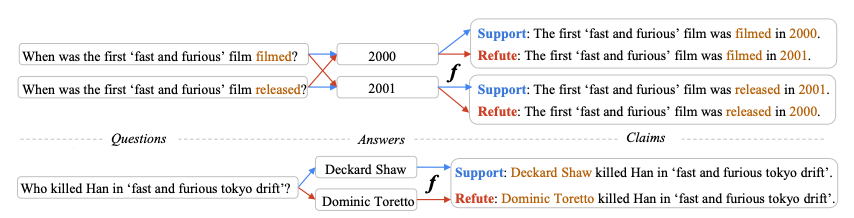
\includegraphics[scale=0.45]{figures/faviq_ambiguity.png}
    \caption{An example of a \texttt{refute} and \texttt{support} claim on FAVIQ, constructed using ambiguity in the information-seeking question and with the use of the reference answer (Deckard Shaw) and the incorrect prediction from DPR. $\boldsymbol{f}$ is a T5 model that transforms question-answer pairs to claims.~\cite{faviq}.}
    \label{fig:faviq1}
\end{figure}

FaVIQ is composed from two sets. The first set, denoted as the \texttt{A set}, consists of claims that were created with ambiguous questions and their disambiguation. The second set is labeled as the \texttt{R set} and consists of claims that were created with reference answer for the \texttt{support} claim and the incorrect prediction from the Dense Passage Retrieval (DPR)~\cite{DPR} model for \texttt{refute} claim. The claims are then generated by T5 model. The statistics of the \texttt{R set} and \texttt{A set} are shown in table~\ref{tab:faviq1}.

\begin{table}[h]
    \centering
    \begin{tabular}{ccccc}
        \hline
         &  & Total & Support & Refute \\
        \hline
        \multirow{2}{*}{Train} & A & 17,008 & 8,504 & 8,504 \\
         & R & 140,977 & 70,131 & 70,846 \\
        \hline
        \multirow{2}{*}{Dev} & A & 4,260 & 2,130 & 2,130 \\
         & R & 15,566 & 7,739 & 7,827 \\
        \hline
        \multirow{2}{*}{Test} & A & 4,688 & 2,344 & 2,344 \\
         & R & 5,877 & 2,922 & 2,955 \\
        \hline
    \end{tabular}
    \caption{FaVIQ dataset statistics~\cite{faviq}. \emph{A} includes claims derived from ambiguous questions, while \emph{R} includes claims from regular question-answer pairs.}
    \label{tab:faviq1}
\end{table}

The question-answer pairs were converted into claims using a trained neural model that maps (\texttt{question}, \texttt{answer}) pairs to claims. A claim is marked as \texttt{support} if the pair from which the claim is generated contains the correct answer to the questions, otherwise the claim is marked as \texttt{refuted}. The model was firstly \texttt{pre-trained} on very similar dataset with thousands of examples and then \texttt{fine-tuned} using a dataset of 250 valid and invalid question-answer pairs that were manually converted. The T5-3B model~\cite{T5} was then trained using 150 statements for training and 100 statements for validation.

In this work, the same methodology is followed in converting QA datasets to Fact-Checking, however, disambiguated questions are not used. This work is based on the system called CORA~\cite{mDPR}. The system returns top-K documents for the question and then generate the answer based on these documents. The data from~\cite{faviq} was used for training the T5 and mT5 model to generate claims.
% \noindent Příklad vytvoření QA do fact checking (TODO)

% ################################################################################################################################################################################

\section{TyDi QA}
The typologically diverse question answering dataset (TyDi QA) \cite{tydiqa} is a dataset that consists of 11 typologically diverse languages with 204 thousands question-answer pairs. Of these, 167 thousands are one-way annotated, to be used for training, and 37 thousands are 3-way annotated, comprising the dev and test sets shown in table~\ref{tab:tydiqa1}.

\begin{table}[h]
    \centering
    \begin{tabular}{l|c|c}
        \textbf{Language} & \textbf{Train} & \textbf{Dev} \\
         & (1-way) & (3-way) \\
        \hline 
        English & 9,211 & 1031 \\
        Arabic & 23,092 & 1380 \\
        Bengali & 10,768 & 328 \\
        Finnish & 15,285 & 2082 \\
        Indonesian & 14,952 & 1805 \\
        Japanese & 16,288 & 1709 \\
        Kiswahili & 17,613 & 2288 \\
        Korean & 10,981 & 1698 \\
        Russian & 12,803 & 1625 \\
        Telugu & 24,558 & 2479 \\
        Thai & 11,365 & 2245 \\
        \hline
        \textbf{Total} & \textbf{166,916} & \textbf{18,670} \\
    \end{tabular}
    \caption{Number of samples from each language represented in the dataset~\cite{tydiqa}.}
    \label{tab:tydiqa1}
\end{table}

Due to its typological diversity, the QA abilities of the model are tested in many distinctive cultural settings. To provide a realistic information-seeking task and avoid priming effects, the questions were written by people who wanted to know the answer but did not yet know the answer. This was achieved by presenting the person with a short prompts consisting of the first 100 characters of Wikipedia articles. After reading it, the person needed to ask a question to which they wanted to know the answer, but this information was not represented in the short prompts. Annotators were asked to provide a question about anything interesting that came to mind, no matter how unrelated to the topic. This allows annotators even more freedom to ask about topics that really interest them, including topics not covered in the Wikipedia articles shown in table~\ref{tab:tydiqa2}. The data are collected directly in each language without the use of translation.

\begin{table}[h]
    \centering
    \begin{tabular}{rl}
        \hline
        Article: & Apple is a fruit... \\
        Question: & What disease did Steve Jobs die of?\\
        \hline
    \end{tabular}
    \caption{Example showing the part of an Wikipedia prompts and a possible question based on the Wikipedia prompts \cite{tydiqa}.}
    \label{tab:tydiqa2}
\end{table}

The dataset contains 10 languages: \emph{English}, \emph{Arabic}, \emph{Bengali}, \emph{Finnish}, \emph{Indonesian}, \emph{Japanese}, \emph{Kiswahili}, \emph{Korean}, \emph{Russian}, \emph{Telugu}, \emph{Thai}.

Each question was then matched with a Wikipedia article by searching for the question text in Google search, restricted to the Wikipedia domain for each language, and then the annotators selected the top-ranked result. The top-ranked result had to be selected based on whether the Wikipedia article contained the answer to the question or whether the question could not be answered using any article (or that no single passage is a satisfactory answer). If such a passage is found annotators were then asked to select the minimum response. Most often, the answer is a few words, but in some cases can span most of a sentence.

% \noindent \textbf{tabulka poctu dat z 1-one way a 3-way (TODO)}

% ################################################################################################################################################################################

\section{XOR-TyDi QA}
The Cross-lingual Open Retrieval Question Answering (XOR-TyDi QA) dataset~\cite{xortydiqa} is a collection of multilingual question-answer pairs that was created for development and evaluation of cross-lingual open-domain QA models. The dataset TyDi QA contains only answers of the same language. Unlike TidyQA, the dataset XOR-TyDi QA was built on questions from the pairs that are lacking same-language answers. Thus the dataset contain questions paired with target documents and answers in English only. These pairs are unanswerable in original dataset. XOR-TyDi QA includes 40k information-seeking questions from across 7 diverse non-English languages: \emph{Arabic}, \emph{Bengali}, \emph{Finnish}, \emph{Japanese}, \emph{Korean}, \emph{Russian} and \emph{Telugu} shown in Table \ref{tab:size}.

\begin{table}[ht]
    \centering
    \begin{tabular}{c|ccccccc}
        Language & Ar & Bn & Fi & Ja & Ko & Ru & Te \\
        \hline
        Size & 20,379 & 5,704 & 12,110 & 9,564 & 5,847 & 11,218 & 8,196
    \end{tabular}
    \caption{Dataset size of the XOR-TYDI QA corpus.}
    \label{tab:size}
\end{table}

The question-answer pairs in the XOR-TyDi QA dataset were collected from Wikipedia articles as it was derived from TyDI QA dataset. The data was human curated and annotated to ensure a high level of quality and relevance. The professional translation service Gengo4 was used to translate all collected questions into English. As named entities were crucial for quality control, translators were instructed to translate them carefully by searching for common English translations from the English Wikipedia or other external sources. Manual quality assessments by native speakers were performed on 50 sample translations, and more than 95\,\% of the translations were found to be correct.

\begin{table}[ht]
    \centering
    \begin{tabular}{c|ccc}
        Language & Train & Dev & Test \\
        \hline
        \hline
        Ar & 18,402 & 708 & 1,269 \\
        Bn & 5,010 & 427 & 267 \\
        Fi & 9,768 & 615 & 1,727 \\
        Ja & 7,815 & 433 & 1,316 \\
        Ko & 4,325 & 371 & 1,151 \\
        Ru & 9,290 & 568 & 1,360 \\
        Te & 6,759 & 351 & 1,086
    \end{tabular}
    \caption{Dataset size of the XOR-TYDI QA corpus splited into sets.}
    \label{tab:stats}
\end{table}

To evaluate the performance of models on the XOR-TyDi QA dataset, the data was divided into a training set, a validation set, and a test set that is shown in Table \ref{tab:stats}. Models were trained on the training set and their performance was evaluated on the validation and test sets.

% ################################################################################################################################################################################

\section{Other datasets}
In addition to X-Fact, there are many other datasets~\cite{fever}\cite{politifact}\cite{covert}\cite{fakenewsnet}\cite{liar} that are designed to support training of modern models. However, most of the datasets, are created in English only and there is quite a small spectrum that deals with multilingual datasets.

One of the many datasets, for example, is the FEVER: Fact Extraction and VERification dataset~\cite{fever}. It consists of 185,445 statements created by modifying sentences extracted from Wikipedia and then verified without knowledge of the sentence from which they were derived. Claims are classified by annotators as \texttt{Supported}, \texttt{Refuted} or \texttt{NotEnoughInfo}. For the first two classes (Supported and Refuted), the annotators also labeled the sentences constituting the necessary evidence for their judgment, which is one of the key shortcomings of the X-Fact dataset. However, the dataset is constructed in English only.

Another dataset is, for example, the Politifact dataset. This is a high-quality dataset that collects data from the PolitiFact website~\cite{politifact}. The dataset contains 21,152 passages that are checked by professional fact-checkers. The dataset is expanded every year with additional data. All passages are divided into 6 categories, namely: \texttt{true}, \texttt{mostly true}, \texttt{half true}, \texttt{mostly false}, \texttt{false}, and \texttt{pants on fire}. It also lists the sources where the statement appeared, which can be crucial for gaining different insights on fact-checking.

There are other datasets \cite{covert}\cite{fakenewsnet}\cite{liar} that deal with fact-checking, but to the best of the author's knowledge no other multilingual datasets have been published. Nowadays, it is important to emphasize multilingual datasets as information/disinformation is disseminated beyond the boundaries of the language in which the disinformation originated\footnote{\url{https://eufactcheck.eu/}}.

% ################################################################################################################################################################################
% ################################################################################################################################################################################

\chapter{Information retrieval}\label{c4}
Ranking retrieval is a process of ordering a set of documents in response to a user query in such a way that the most relevant documents appear at the top of the list. Formally, given a query $q$ and a collection of documents $D = \{d_1, d_2, ..., d_n\}$, the ranking retrieval function $f(q,D)$ assigns a score to each document $d_i$ in $D$, such that the documents are sorted in descending order of their scores, and the top-ranked documents are considered the most relevant to the query.

Information retrieval models are statistical models used to represent the process of retrieving relevant information from a large collection of documents or other data sources. The goal of information retrieval models is to assist users in finding the most relevant documents or information in response to a specific query.

There are various information retrieval models, but some of the most common include the Boolean model~\cite{BM25}, the vector space model~\cite{vectore_space}, the probabilistic model, the latent semantic indexing (LSI) model~\cite{LSI}, and neural network models~\cite{nn_models}. The Boolean model uses Boolean logic to match documents to queries. The vector space model represents documents and queries as vectors in a high-dimensional space, where each dimension corresponds to a term in the vocabulary. It computes the similarity between them using measures such as cosine similarity. 
\begin{quotation}
    Cosine similarity measures the similarity between two vectors of an inner product space. It is measured by the cosine of the angle between two vectors and determines whether two vectors are pointing in roughly the same direction. It is often used to measure document similarity in text analysis. \cite{cosine_similarity}
\end{quotation}
The probabilistic model, on the other hand, uses probabilistic techniques to rank documents based on the likelihood that they are relevant to a query, taking into account factors such as term frequency and document length. The LSI model uses singular value decomposition to identify hidden relationships between terms in the corpus, while neural network models such as convolutional neural networks (CNN)~\cite{cnn} and transformers~\cite{transformer} show promising results when applied to information retrieval tasks. One of the transformer-based document retrieval models is Multilingual Dense Passage Retrieval (mDPR)~\cite{mDPR}. It is a dense retrieval method that encodes the query and documents into dense representations using pre-trained multilingual language models such as mBERT~\cite{mbert}, and then compares the query and documents in a vector space to retrieve the most relevant passages.

Information retrieval models can also be divided into sparse and dense models based on their approach to representing and matching textual data. Sparse information retrieval models, such as the classical Boolean model, represent textual data as binary vectors that indicate whether or not each term occurs in a document. In contrast, dense information retrieval models use continuous, dense representations of textual data that capture more subtle information about the relationships between terms, that is the key advantages.

Information retrieval models are essential in natural language processing and enable effective retrieval over large text corpus.

% ################################################################################################################################################################################

\section{Dense passage retrieval}
Dense Passage Retrieval (DPR)~\cite{DPR} is a method of dense retrieval model used for information retrieval tasks that involves retrieving relevant passages of text from a large corpus. DPR encodes both the query and documents into dense representations using pre-trained transformer models such as BERT~\cite{bert}, and then matches them in a vector space to retrieve the most relevant passages.

Dense passage retrieval uses a dense encoder $E_P(\cdot)$ which maps any input passage to a \emph{d}-dimensional real-valued vectors and builds an index for all the \emph{M} passages that will be used for retrieval:

\begin{equation}
    E_P(\mathbf{x}, \mathbf{m}) : (\mathbb{R}^{n \times d}, \mathbb{R}^{n \times 1}) \rightarrow \mathbb{R}^d
\end{equation}
where $\mathbf{x} \in \mathbb{R}^{n \times d}$ is a matrix representing the input document tokens, $\mathbf{m} \in \mathbb{R}^{n \times 1}$ is a vector representing the attention mask for the input tokens, and $E_P(\mathbf{x}, \mathbf{m}) \in \mathbb{R}^d$ is the output vector representing the encoded document.

A different encoder $E_Q(\cdot)$ is applied at the run-time, which maps the input query to a $d$-dimensional vector and obtains the $k$ passages that are closest to the query vector:
\begin{equation}
    E_Q(\mathbf{x}, \mathbf{m}) : (\mathbb{R}^{n \times d}, \mathbb{R}^{n \times 1}) \rightarrow \mathbb{R}^d
\end{equation}
where $\mathbf{x} \in \mathbb{R}^{n \times d}$ is a matrix representing the input query tokens, $\mathbf{m} \in \mathbb{R}^{n \times 1}$ is a vector representing the attention mask for the input tokens, and $E_Q(\mathbf{x}, \mathbf{m}) \in \mathbb{R}^d$ is the output vector representing the encoded query.

These encoders are two different BERT networks with output on the token [CLS], so \emph{d}\,$=$\,768. The input tokens are first tokenized and passed through the BERT model, which consists of multiple transformer layers. Each transformer layer applies self-attention and feed-forward neural networks to the input tokens to compute a contextualized representation of each token. The output of the final transformer layer is then used as the encoded representation of the input document or query.

In particular, the $E_P$ takes as input a matrix $\mathbf{x}$ of document tokens and a vector $\mathbf{m}$ of attention masks, where each element of $\mathbf{m}$ is either 0 or 1 to indicate whether a corresponding token should be masked out or not. The $E_P$ passes $\mathbf{x}$ and $\mathbf{m}$ through the BERT model to obtain a matrix of contextualized token representations. The attention mask is used to ensure that the masked tokens do not affect the output of the BERT model. The matrix of contextualized token representations is then aggregated into a single vector representation of the document using an attention mechanism.

Similarly, the $E_Q$ takes as input a matrix $\mathbf{x}$ of query tokens and a vector $\mathbf{m}$ of attention masks. The $E_Q$ passes $\mathbf{x}$ and $\mathbf{m}$ through the same BERT model to obtain a matrix of contextualized token representations. The $E_Q$ also uses an attention mechanism to aggregate the matrix of contextualized token representations into a single vector representation of the query.

The similarity is defined as a dot product between the query vector and the document vector:

\begin{equation}
    sim(q, p) = E_Q(q)^TE_P(p).
\end{equation}

\subsection*{Training}
Encoder training is done to maximize the cosine similarity between the query and relevant passages and minimize the cosine similarity between the query and irrelevant passages. The goal is to create a vector space that contains relevant pairs of question and passage vectors with smaller distance (i.e., higher similarity) than the irrelevant ones. Let $D = \{\langle q_i, p_i^+, p_{i,1}^-, \dots , p_{i,n}^-\rangle\}_{i=1}^m$ be the training data that contains \emph{m} instances. Each instance contains one question $q_i$ and one positive passage $p_i^+$ along with \emph{n} negative passages $p_{i,j}^+$ shown in table~\ref{tab:dpr}. The loss function is then optimized as the negative log-likelihood of the positive passage:

\begin{equation}
    L(q_i, p_i^+, p_{i,1}^-, \dots , p_{i,n}^-) = -\operatorname{log}\frac{e^{sim(q_i,p_i^+)}}{e^{sim(q_i,p_i^+)}+\sum_{j=1}^n e^{sim(q_i,p_{i,j}^-)}}. \label{eq:dpr}
\end{equation}

\begin{table}[h]
    \centering
    \begin{tabular}{lp{7cm}}
        \hline
        Question: &  What is the capital of France? \\
        \hline
        Positive passage: & The capital of France is Paris, one of the most famous cities in the world, known for its art, fashion, and cuisine. \\
        \hline
        Negative passage 1: & France is a beautiful country located in Western Europe. It is home to a diverse range of landscapes, from the snowy peaks of the Alps to the sandy beaches of the Mediterranean coast. \\
        \hline
        Negative passage 2: & The Eiffel Tower is a famous landmark in France that attracts millions of visitors every year. It was built in the late 19th century as part of a World's Fair held in Paris. \\
        \hline
    \end{tabular}
    \caption{Example of a query, positive passages and negative passages.}
    \label{tab:dpr}
\end{table}

For retrieval problems, it is often the case that positive examples are available explicitly, while negative examples must be selected from an extremely large set. Relevant passages to the question may be listed in the QA dataset or may be found by using the answer. All other passages could be considered irrelevant in this case. Therefore, negative passages were selected using three different procedures:
\begin{enumerate}
    \item the first procedure, the so-called \emph{random procedure}, was to select a random passage from the corpus,
    \item the second procedure, the so-called \emph{BM25 procedure}, was to select passages that were returned as best by BM25 model~\cite{BM25} and contain most of the question tokens but do not contain the answer,
    \item the last procedure, the so-called \emph{in-batch negatives}, consisted of selecting a positive passage and pairing it as negative with another question that appeared in the training set.
\end{enumerate}

Using \emph{in-batch negatives} has proven to be an effective approach because it's an easy and memory-efficient way to reuse negative examples already in a batch rather than creating new ones. The experiments in DPR paper~\cite{DPR} led to the conclusion that combining the second and third approaches is the best approach. That is, they took the negative passages from the \emph{in-batch negatives} and added 7 negative passages from the \emph{BM25 procedure}.

% ################################################################################################################################################################################

\section{Multilingual dense passage retrieval}
Multilingual dense passage retrieval \cite{mDPR} (mDPR) is a retrieval model used for information retrieval tasks. It is a variant of the dense passage retrieval \cite{DPR} (DPR) model and is designed to be multilingual and cross-lingual, meaning that it can handle queries and documents in multiple languages. mDPR encodes both the query and the documents into a dense representation in the same way as DPR. However, since mDPR is designed as a multilingual model, it uses multilingual BERT (mBERT)~\cite{mbert}.

mDPR is used to rank passages based on their relevance to a given query. It does so by representing each passage as a dense vector, using a combination of language models and transformer networks.

To rank passages for a given query, mDPR uses the following basic equation:

\begin{equation}
    \operatorname{Score}(\mathbf{P}, \mathbf{Q}) = \text{cosine\_similarity}(\mathbf{P}, \mathbf{Q}),    
\end{equation}

\noindent where \emph{P} is the dense vector representation of the passage, \emph{Q} is the dense vector representation of the query and \texttt{cosine\_similarity} is a measure of the similarity between two vectors, calculated as the dot product of the vectors divided by the product of their magnitudes:

\begin{equation}
    \text{cosine\_similarity}(\mathbf{P}, \mathbf{Q}) = \frac{\mathbf{Q} \cdot \mathbf{P}}{\lVert \mathbf{Q} \rVert \lVert \mathbf{P} \rVert} = \frac{\sum_{i=1}^{n} Q_i P_i}{\sqrt{\sum_{i=1}^{n} Q_i^2} \sqrt{\sum_{i=1}^{n} P_i^2}}.
\end{equation}

mDPR can handle queries by taking into account the full context of the passages it is ranking, in addition to evaluating their relevance to a given query. This makes it an attractive option for tasks such as question answering, where the meaning of the query may not be clear from the individual terms alone.

mDPR has been shown to be an effective method for ranking passages based on their relevance to a given query. It has been compared to other retrieval models, including Okapi BM25, and has demonstrated strong performance in a number of different benchmarks~\cite{BM25}. As such, it is often used as a baseline method for evaluating the performance of other retrieval models and has the potential to be a useful tool in a variety of information retrieval tasks.

\subsection*{Comparsion of mDPR with DPR}
Let $D = \{\langle q_i, p_i^+, p_{i,1}^-, \dots , p_{i,n}^-\rangle\}_{i=1}^m$ be \emph{m} training instances. Each instance consists of a question $q_i$, a passage that answers the question $p_i^+$ (a positive passage),
and \emph{n} passages that do not answer the question $p_{i,j}^-$ (negative passages). The mDPR model is then trained in the same way as the DPR model with equation~\ref{eq:dpr}, as described in the section on DPR.

DPR is originally initialized with the English BERT~\cite{bert}. For multilingual search and to take advantage of cross-language transfer, the mDPR model was initialized with mBERT~\cite{mbert}, while all other aspects of training remained the same~\cite{mDPR_training}.

Several works~\cite{mdpr_ref1}\cite{mdpr_ref2}\cite{mdpr_ref3}\cite{mdpr_ref4} have shown that monolingual BERT models can be more efficient than mBERT in various natural language processing tasks, but the gains are not consistent. In a publication~\cite{mDPR_training}, the results of the comparison of the monolingual model with the multilingual model were published. The results showed that it is possible that there are ``better'' monolingual BERT models for the target language than mBERT. However, the advantage of the mBERT model is that it can be easily pre-finetuned by using the MS MARCO dataset~\cite{msmarco} and leveraging datasets from other languages.  Obviously, for monolingual (non-English) BERT, it is no longer possible to pre-fine-tune the model on MS MARCO. A recommendation is included in the publication:
\begin{quotation}
    Using a monolingual BERT backbone can yield a model that is more effective than using mBERT, but the monolingual model is not consistently better. Thus, it seems “safer” to just use mBERT as the backbone. \cite{mDPR_training}
\end{quotation}

A comparison of the results of all experiments can be found in the publication~\cite{mDPR_training}. Part of the results table is presented in Table~\ref{tab:mdpr_results}.

\begin{table}[h]
    \centering
    \begin{tabular}{l|ccccc}
        \hline
        Language & Ar & En & Fi & Id & Ko \\
        \hline
        multilingual DPR &  0.900 & 0.841 & 0.856 & 0.860 & 0.785 \\
        monolingual DPR & 0.894 & 0.805 & 0.893 & 0.888 & 0.820 \\
        \hline
    \end{tabular}
    \caption{Results from the publication~\cite{mDPR_training} with a performance metric Recall@100.}
    \label{tab:mdpr_results}
\end{table}

To achive this results monolingual DPR was trained for all languages separately. The languages represented in the experiment were: \emph{Arabic}, \emph{English}, \emph{Finnish}, \emph{Indonesian} and \emph{Korean}. Multilingual DPR was trained for all languages. The models were trained in 40 epochs with the corresponding training data (single or multiple languages) with 128 batch size without using transaltions. The monolingual DPR models were trained on data used from Mr. TYDI dataset~\cite{mrtydi}. The multilingual DPR was trained on MS MARCO dataset. The Recall@100 metric was then used for the evaluation of the models. Recall@100 is a metric used to evaluate the performance of information retrieval models. It measures the percentage of relevant documents that are retrieved among the top 100 results for a given query.

% ################################################################################################################################################################################
% ################################################################################################################################################################################

\chapter{Proposed system for dataset conversion}\label{c5}
Following text is based on the findings presented in paper~\cite{faviq} about creation of a multilingual dataset for fact verification from an existing question-answering dataset. The main goal was to see if it is possible to automatically create a challenging dataset without help of human translators and annotators.

This work also goes trough this topic with additional comparison where two different approaches for dataset creation are attempted. The XOR-TyDi QA dataset was used for the conversion. The dataset consist of 7 languages: \emph{Arabic}, \emph{Bengali}, \emph{Finnish}, \emph{Japanese}, \emph{Korean}, \emph{Russian} and \emph{Telugu}. This work assumes that the question-answer pairs are in the same language. It is proceed in the way when someone asks a question, he receives the answer in the same language in which the question was asked. However, this may not always be true for the evidence that contains the necessary information for the model to answer the question. The evidence may be in a different language than the language in which the question is represented. Even so, the model should be able to take the information from the other language and then return the answer in the desired language shown in Figure~\ref{fig:other_language}.

\begin{figure}[H]
    \centering
    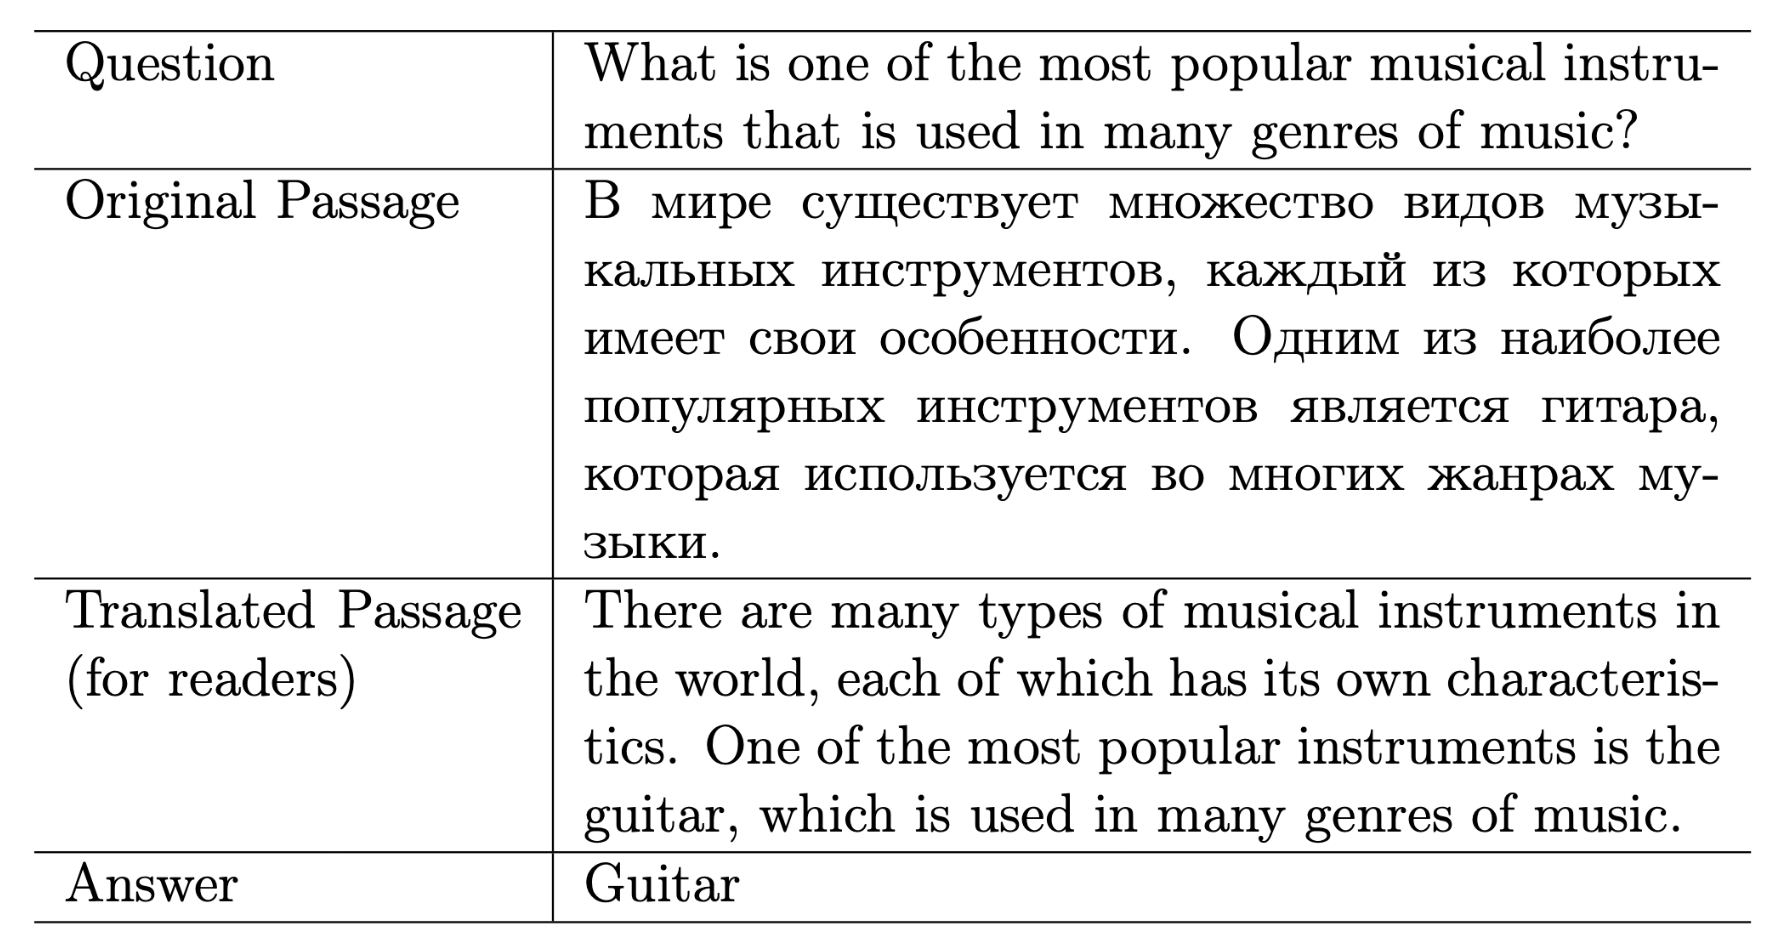
\includegraphics[scale=0.2]{figures/example1.png}
    \caption{Example of question in English an the information in the Russian language with the generated answer in English.}
    \label{fig:other_language}
\end{figure}

% \begin{table}[H]
%     \centering
%     \begin{tabular}{p{3.22cm}|p{8cm}}
%         \hline
%         Question & What is one of the most popular musical instruments that is used in many genres of music? \\
%         \hline
%         Original Passage & \textcyrillic{В мире существует множество видов музыкальных инструментов, каждый из которых имеет свои особенности. Одним из наиболее популярных инструментов является гитара, которая используется во многих жанрах музыки.} \\
%         \hline
%         Translated Passage (for readers) & There are many types of musical instruments in the world, each of which has its own characteristics. One of the most popular instruments is the guitar, which is used in many genres of music. \\
%         \hline
%         Answer & Guitar \\
%         \hline
%     \end{tabular}
%     \caption{Caption}
%     \label{tab:my_label}
% \end{table}

\section{Answer generation}


\subsection{Data}
The data which were used to return the documents are from the February 2019 Wikipedia dumps of 13 diverse languages contain all XOR-TyDi QA languages~\cite{mDPR}. These 13 languages have a large number of Wikipedia articles and a variety of both Latin and non-Latin scripta continua. The data were extracted from Wikipedia using wikiextractor~\cite{wikiextractor} and then each article was splitted into 100-token segments. In~\cite{mDPR} they also filtered out the short articles with fewer than k (i.e., k = 20 in the paper) tokens resulting in 43.6M passages in total.

\subsection{mDPR}
One of the main part of the proposed system is article document retrieval. The implementation of the mDPR model taken from~\cite{mDPR} covered all the steps described in this subsection. The mDPR produced dense embeddings of a question and all multilingual passages, thereby retrieving passages across all languages.

In order to answer a question, we need to find the record in which the answer to the question is located. This is the document retrieval task to returns a certain number of the most relevant documents in which the answer might be located. These documents are returned in different languages. The documents are then evaluated based on an \texttt{exact match score} metric (explained in Section~\ref{exact_match}) with the correct answer, since the answers are represented in the dataset from which the question is taken. Thus, the label ``has\_answer'' was added to each sample to indicate whether the target answer is present in the document.

% This was all done with the implementation of the mDPR model, that is a multilingual document retrieval. The mDPR produced dense embeddings of a question and all multilingual passages, thereby retrieving passages across all languages.

\subsection{Generation of positive and negative\\question-answer-passage triplets}\label{pos_neg_answers}
The generation model (mGEN) taken from~\cite{mDPR} was trained to output an answer in the target language based on the retrieved multilingual passages. The resulting dataset must contain not only positive answers but also negative answers. They were created in the FaVIQ paper~\cite{faviq} using two approaches, particularly with the help of ambiguous questions and documents retrieved by document retrieval. In this work, only the approach with help of documents retrieved mDPR was used.

Let $Q^* = \{q_1, q_2,..., q_n\}$ be all questions and $A^* = \{a_1^+, a_2^+,..., a_n^+\}$ be all answers to the questions from the XOR-TyDi QA dataset~\cite{xortydiqa}.

% $A^* = \{a_1^+, a_2^+,..., a_n^+\}$ pozitivni odpovedi z XOR TyDi QA

% $Q^* = \{q_1, q_2,..., q_n\}$ pozitivni odpovedi z XOR TyDi QA

% $P^+_i = mDPR(q_i)$ navracene dokumenty z mDPR pro spravnou odpoved

% $P^-_i = mDPR(q_i)$ navracene dokumenty z mDPR pro spatnou odpoved

% $a^+ = mGEN(q_i, P^+_i)$ generovani spravne odpovedi

% $a^- = mGEN(q_i, P^-_i)$ generovani spatne odpovedi

% $F1(a^-, A_i^*) = 1$ pokud rovno 1 tak odpoved je stejna jak v XOR TyDi QA a tedy pravdiva, pokud se nerovna 1 tak odpoved neni obsazena v XOR a tedy muze byt povazovana za nepravdivou (pouze pro spatne odpovedi)

% $(a^-, q_i)$ question-answer pair

% $EM(a^+, P^+_i) = 1$ pasaz s evidenci pro spravnou odpoved

% $EM(a^-, P^-_i) = 1$ pasaz s evidenci pro spatnou odpoved

\subsubsection*{Positive triplets}
To generate a positive answer $a^+$, the questions $q_i$ were submitted to mDPR, which retrieved the top 100 documents. Let $P$ be all passages returned from mDPR for the question $q_i$. Since mGEN was trained with a set of 15 documents, these 100 documents denoted as $P$ retrieved by mDPR were then post-processed in the way that only the top 15 documents that have the ``has\_answer'' label set to \emph{True} are taken into mGEN. If there were less than 15 documents with a label set to True, the sample was not considered in further triplet formation. Based on these documents mGEN then generates an answer $a^+$ for each question $q_i \in Q^*$ with the resulting scores shown in table~\ref{tab:mgen_positive}.

The generated answer $a^+$ was then postprocessed with a goal to eliminate answer that was not present in any of the passages $P$ retrieved by mDPR. Therefore, let $\operatorname{EM}(a^+, P_i)$ be the exact match score metric~\ref{exact_match} that calculates the score with each passage $P_i \in P$ returned from mDPR. The $\operatorname{EM}$ was ten evaluated in the way $\operatorname{EM}(a^+, P_i) = 1$. If the result score was equal to 1 the answer $a^+$ was presented in the passage $P_i$. The answer $a^+$ is paired with the passage $P_i$ and question $q_i$. This resulted into formation of the final positive triplet. Rest of the passages in $P$ were not used in the final output. Samples that had no $P_i$ passage that contained the answer $a^+$ information were not converted to the final positive triplet. The results are shown in table~\ref{tab:mgen_positive}.

\begin{table}[h]
    \centering
    \begin{tabular}{l|lccc}
        \hline
         Dataset & Postprocess & Number of Samples & F1 score & EM Score \\
        \hline
        \multirow{3}{*}{Dev} & Original & 3473 & 46.08\,\% & 34.35\,\% \\
         &  EM procedure & 1145 & 61.09\,\% & 49.78\,\% \\
         \hline
        \multirow{3}{*}{Train} & Original & 61340 &  54.36\,\% & 42.96\,\% \\
         & EM procedure & 29751 &  73.69\,\% & 62.91\,\% \\
        \hline
    \end{tabular}
    \caption{Results using F1 and EM metrics (explained in Section~\ref{exact_match}) from the postprocess procedure for positive answers. The column named ``Postprocess'' indicates the specific procedure step. In the EM procedure the data was filtered in the way to eliminate answers that did not contain an passage with the evidence of the answer.}
    \label{tab:mgen_positive}
\end{table}

\subsubsection*{Negative triplets}
To generate a negative answer $a^-$, the same procedure was followed as for a positive answer $a^+$, with the only difference that the top 15 passages $P$ that have the ``has\_answer'' label set to \emph{False} are taken to generate the answer. The label set to false means they do not contain any answer match. Based on these documents mGEN generated an answer $a^-$ for each question $q_i \in Q^*$ with the resulting scores shown in table~\ref{tab:mgen_negative}.

The generated answer $a^-$ was then postprocessed with a goal to eliminate answer in the way $\operatorname{F1}(a^-, A^*) = 1$. This score indicates that generated answer $a^-$ was likely correct, as it was included in the original dataset answers $A^*$ and since the purpose of this answer was to be incorrect, it was not considered in further triplet formation. Then for each answer $a^-$ the $\operatorname{EM}$ was ten evaluated for each passage $P_i \in P$ in the way $\operatorname{EM}(a^-, P_i) = 1$. If the $\operatorname{EM}$ score was equal to 1 the answer $a^-$ was presented in the passage $P_i$. The answer $a^-$ was paired with the passage $P_i$ and question $q_i$. This resulted into formation of the final negative triplet. Rest of the passages $P$ were not used in the final output. Samples that had no $P_i$ passage that contained the answer $a^-$ information were not converted to the final negative triplet. The results are shown in table~\ref{tab:mgen_negative}.

\begin{table}[H]
    \centering
    \begin{tabular}{l|lccc}
        \hline
         Dataset & Postprocess & Number of Samples & F1 score & EM Score \\
        \hline
        \multirow{3}{*}{Dev} & Original & 3473 & 17.72\,\% & 11.66\,\% \\
         &  F1 procedure & 3068 & 6.86\,\% & 0.00\,\% \\
         &  EM procedure & 1080 & 9.01\,\% & 0.00\,\% \\
         \hline
        \multirow{3}{*}{Train} & Original & 61340 &  25.50\,\% & 19.33\,\% \\
         & F1 procedure & 49452 &  7.59\,\% & 0.00\,\% \\
         & EM procedure & 18037 &  9.13\,\% & 0.00\,\% \\
        \hline
    \end{tabular}
    \caption{Results using F1 and EM metrics (explained in Section~\ref{exact_match}) from the postprocess procedure for negative answers. The column named ``Postprocess'' indicates the specific procedure step. In the F1 procedure the data was filtered in the way to eliminate answers that was likely correct as they were included in the original dataset. In the EM procedure the data was filtered in the way to eliminate answers that did not contain an passage with the evidence of the answer.}
    \label{tab:mgen_negative}
\end{table}

\section{Conversion system} \label{t5_proposed}
The mGEN model only generated a set of correct and incorrect answers to the question, but the final result to be achieved in this work is to create a multilingual fact-checking dataset. So the questions and answers need to be converted into the claims. Based on the question the mGEN generates the answer. As a result we have a question-answer pairs. From these pairs, the T5 model~\ref{T5} was trained to generate a claim. The question contains information about what the answer specifically refers to and the answer itself is the information we want to transfer to the claim. From this point the execution flow was split into two approaches. The first approach was to train a multilingual T5 model~\cite{mt5} (mT5) with the use of the dataset that has the question-asnwer pairs in all considered languages. The second apporach is to train the monolingual T5 model~\cite{T5} with dataset that contains only the data in English language.

\subsection*{Training}
The training of these two models was done using data that were collected from the original paper FaVIQ~\cite{faviq}. The data consist of three datasets. The first dataset was used for pre-training and has 60k examples of the question-answer pairs and the target outputs that stand for the target claims. It includes also 10k examples for validation~\cite{faviq}. The dataset was collected from one of the authors of the Faviq paper~\cite{faviq}. The sample from the pre-training dataset is shown in table~\ref{tab:t5_dataset}. 

\begin{table}[H]
    \centering
    \begin{tabular}{lp{8cm}}
        \hline
        Dataset: & SQuAD \\
        ID: & 570bf0896b8089140040fada \\
        Question: & Why did the committee debate adding a shift function? \\
        Answer: & would allow more than 64 codes to be represented by a six-bit code \\
        Claim: & Committees debated on adding a shift function because it would allow more than 64 codes to be represented by a six-bit code. \\
        \hline
    \end{tabular}
    \caption{Sample from dataset used for pre-training.}
    \label{tab:t5_dataset}
\end{table}

The other two datasets are manually annotated samples in English for the purpose of fine-tuning a monolingual T5 model. The datasets were collected from one of the authors of the Faviq paper~\cite{faviq}. They were created in the same way as \texttt{R Set} and \texttt{A Set} described in section~\ref{seq:faviq}. They consist of the same data structure that was needed for pre-training. Each dataset has the structure of one example as: \emph{question}, \emph{positive answer}, \emph{negative answer}, \emph{positive claim} and \emph{negative claim}. Each dataset has $\approx$~150 samples for training and $\approx$~100 samples for validation. The sample from the fine-tuning dataset is shown in table~\ref{tab:t5_dataset2}. These datasets were used for fine-tuning of the models. There was no difference between positive and negative question-answer pairs that were used for fine-tuning, as mentioned by the author of these datasets. Thus the samples from both datasets were separated into two examples (positive and negative). Therefore, for fine-tuning task the dataset had 600 samples for training (each dataset consist of 150 samples of positive and negative example, i.e. $2^2\cdot150$) and 400 samples for validation (each dataset consist of 100 samples of positive and negative example, i.e. $2^2\cdot100$). The datasets were created in english language. Therefore, theses datasets need to be translated into all desired languages for training of a multilingual mT5 model.

\begin{table}[H]
    \centering
    \begin{tabular}{lp{7cm}}
        \hline
        Question: & Who was the comedian who said chase me? \\
        Positive Answer: & duncan norvelle \\
        Positive Claim: & duncan norvelle was the comedian who said chase me \\
        Negative Answer: & chevy chase \\
        Negative Claim: & chevy chase was the comedian who said chase me \\
        \hline
    \end{tabular}
    \caption{Sample from dataset used for fine-tuning.}
    \label{tab:t5_dataset2}
\end{table}

\subsection*{English}
The pre-trained model from the huggingface library, namely ``t5-base'', was used for the monolingual T5 English model. The "t5-base" model was pre-trained on the large C4 corpus~\cite{transformer}. The base version of T5 has 220M parameters that can be tuned.

The model was first pre-trained on the first dataset on 10 epochs. One epoch means that the model went through all the samples from the dataset exactly once and tried to predict the correct outputs. Each epoch was run with a batch size of 12, which means that 12 samples from the datasets were taken and computed at a time. The maximum sequence length was set to 256. A loss function was then calculated for each batch and gradients were calculated to update the model weights. Gradient accumulation was also used, meaning that the weights were only updated in some iteration of the training process. The gradient accumulation was set to 3 in this case. It means that every third iteration of training loop updated the model weights. At the end of each pre-training epoch, the checkpoint was evaluated based on the Rouge score, exact match score and F1 metrics~\ref{exact_match}. After 10 epochs, the performance of the model began to fluctuate. Thus, the model was not pre-trained for any further epochs and moved to the fine-tuning phase.

The model was fine-tuned using two other datasets on 900 epochs. The maximum sequence length and the batch size were the same as in pre-training. The gradient accumulation was also set to 3. During fine-tuning, a checkpoint was evaluated every 20 epochs. Fine-tuning was stopped in the 900 epoch, as it became clear that the model was already performing well in manual tests. Manual tests consisted of manually created questions and answers. Tests were used to check that the model generates correct claims.

After training the model, the resulting claims were generated using translation of the questions and answers into English. The model generated claims in English, which were then translated back into the desired language. Translations were made using the machine translation model described below. The model input structure was created by adding the prefixes ``question:'' before the target question and ``answer:'' before the target answer: ``\texttt{question: Who was the comedian who said chase me? answer: duncan norvelle}''. The recommended generation method\footnote{\url{https://huggingface.co/blog/how-to-generate}} from the HuggingFace library was used. The max length of the sequence was set to 256. Generation was based on the beam search~\cite{beamsearch} which reduces the risk of missing hidden high probability word sequences by keeping the most likely ``num\_beams'' of hypotheses at each time step and eventually choosing the hypothesis that has the overall highest probability. The ``num\_beam'' parameter was set to 5. The parameter ``early\_stopping'' was set to True with the ``no\_repeat\_ngram\_size'' parameter set to 3. The ``n-grams'' penalty ensured that no ``n-gram'' (i.e. 3-gram in this case) appears twice by manually setting the probability of next words that could create an already seen ``n-gram'' to 0. The resulting scores for the T5 model are shown in table~\ref{tab:t5_results}.

\subsection*{Multilingual}
For the multilingual T5 model, which was trained for all languages, a pre-trained model ``google/t5-base'' from the huggingface library was used. The base version of mT5 has 580M parameters that can be tuned. To train the model, the datasets collected from one of the authors of FaVIQ paper were translated into all desired languages and then combined into target datasets. 
For training, the same approach as for the T5 model was used, except that only 3 epochs were performed for pre-training and then 900 epochs were used for fine-tuning. The batch size was the same as for T5 training, with the use of gradient accumulation. The difference between the number of pre-training epochs was due to the size of the training data. Since the original dataset was translated into all target languages, the size of the training dataset was almost 500,000 samples. The generation method with the same parameters was used as for monolingual T5 English model.

After the training process, the input was passed to the model to generate the claim. The structure of the input to the model was the same as shown in the T5 model except that a prefix for the target language was added: "\texttt{language: en question: Who was the comedian who said chase me? answer: duncan norvelle}". The resulting scores for the mT5 model are shown in table~\ref{tab:t5_results}.

\begin{table}[h]
    \centering
    \begin{tabular}{l|lc}
        \hline
        Model & Metric & Score \\
        \hline
        \multirow{4}{*}{T5} & Rouge-1 & 85\,\% \\
         & Rouge-2 & 78\,\% \\
         & Rouge-L & 84\,\% \\
         & EM & 19\,\% \\
         \hline
        \multirow{4}{*}{mT5} & Rouge-1 & 66\,\% \\
         & Rouge-2 & 51\,\% \\
         & Rouge-L & 61\,\% \\
         & EM & 6\,\% \\
        \hline
    \end{tabular}
    \caption{Evaluation of the trained models based on Rouge and Exact Match score metrics (explained in Section~\ref{exact_match}).}
    \label{tab:t5_results}
\end{table}

As can be seen the T5 model achieved better results than the mT5 model in automatic metrics. This was caused with the bad performance of the translation models as the metrics were calculated on the validation dataset that was used for fine-tuning the mT5 and T5 models. These datasets were firstly translated into all desired languages for the training of the mT5 model.

Therefore two errors are for the bad performance of the mT5 model. The error\#1 is because of translations in some languages did not even reach 50\,\% success rate (described in Section~\ref{human_translation}), therefore the target claims were translated into claims that were not correct prediction in the target language for the model. The error\#2 is that after the translation of the sample into the target language, the question and answer did not represent the same meaning as the translated claim. Thus the mT5 generated relevant claim for the input question and answer but the target claim was different because of the translation. Unfortunately, these are still only hypotheses and experiments have not been performed to explain this problem.

\section{Translation}
The translation was performed using the Helsinki OPUS-MT~\cite{helsinki} described in Section 2.1. For each language, a different model was used. Each model was trained for the target language. Since the Helsinki OPUS-MT lacked a translator model for Korean, a second translator model was used in this work, namely "facebook/m2m100\_1.2B". The model was trained for Many-to-Many multilingual translation and covers Korean as well.

All models were taken from the huggingface library, where the models are already pre-trained for the translation task. Translation is one of the main limitations of this work, as after manual analyses it was found that not all models translated the input to the target language correctly, especially for non-Latin languages. An example of a query translated from English to Telugu and then translated back to English is shown in table~\ref{tab:translation}. On the other hand, the models work well in Latin languages, as can be seen in section~\ref{human_translation}. 

\begin{table}[h]
    \centering
    \begin{tabular}{lp{7cm}}
        \hline
        Original query: & The chicken is afraid of the road. \\
        Translated query: & The cold night's scared.\\
        \hline
    \end{tabular}
    \caption{Example of a translated query from English to Telugu and back to English.}
    \label{tab:translation}
\end{table}

However, the sentences in the original dataset are not that complex and each translator model performed well. The back-translation is evaluated in Section~\ref{human_translation}.

\section{Final dataset}
All the parts that are needed for the final pipeline are described and therefore the final pipeline structure can be interpreted. Both approaches are almost identical except the translation part. For the monolingual approach, the pipeline is shown in figure~\ref{fig:t5}.

\begin{figure}[H]
    \centering
    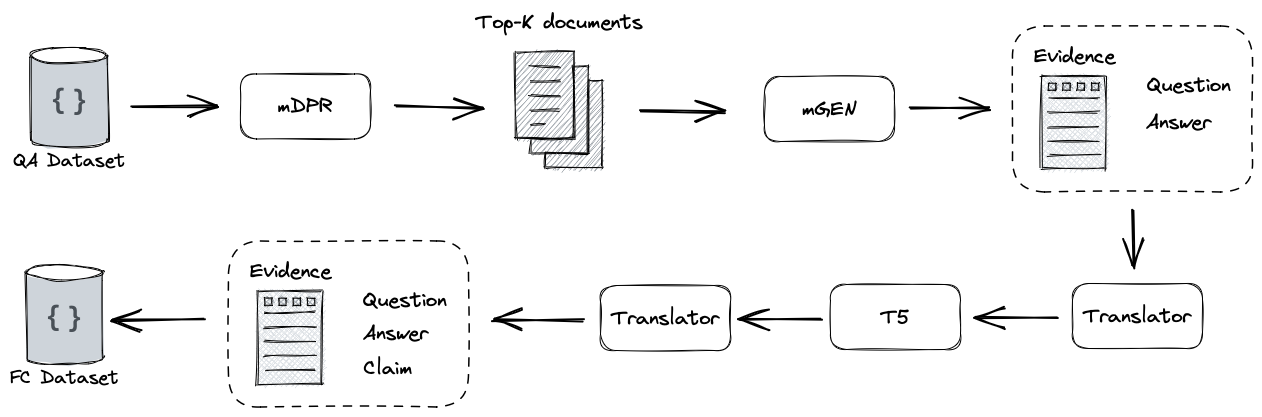
\includegraphics[scale=0.3]{figures/T5.png}
    \caption{Pipeline for the approach with the English T5 model.}
    \label{fig:t5}
\end{figure}

\noindent For the multilingual model the pipeline is shown in figure~\ref{fig:mt5}. 

\begin{figure}[H]
    \centering
    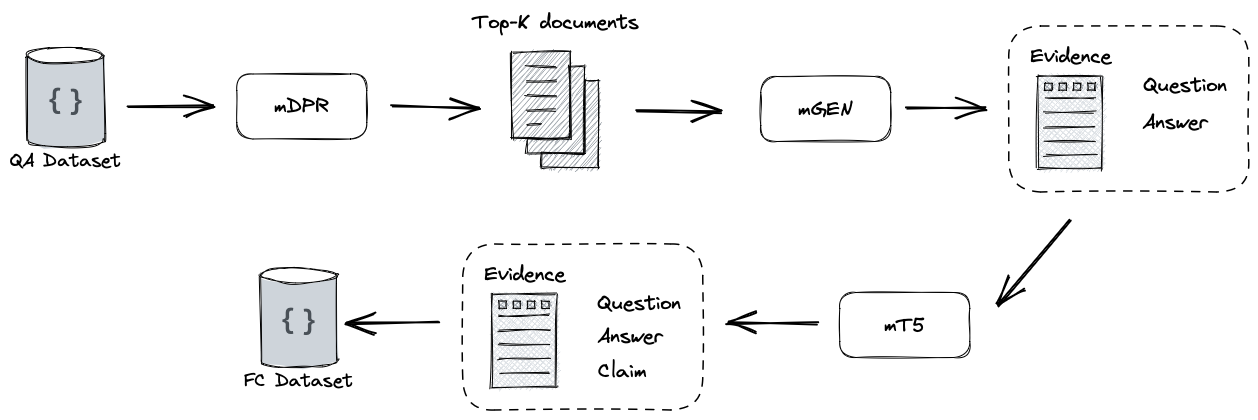
\includegraphics[scale=0.3]{figures/mT5.png}
    \caption{Pipeline for the approach with the multilingual T5 model.}
    \label{fig:mt5}
\end{figure}

As the final result both approaches convert dataset with the same samples and structure. The structure of one sample from the dataset is shown in table~\ref{fig:dataset}. The datasets consists of the validation dataset and the training dataset. The test dataset for final testing was not converted in this work, since in this work there were no evaluations of final fact-checking model that required the test dataset and therefore it was not needed for the experiments. Experiments were performed on the fact-checking model based on TF-IDF and it did not need a test data set to evaluate~\ref{seq:experiments_tfidf}. However, to convert also the test dataset is straightforward since all the required parts for the creation were described.

\begin{figure}[H]
    \centering
    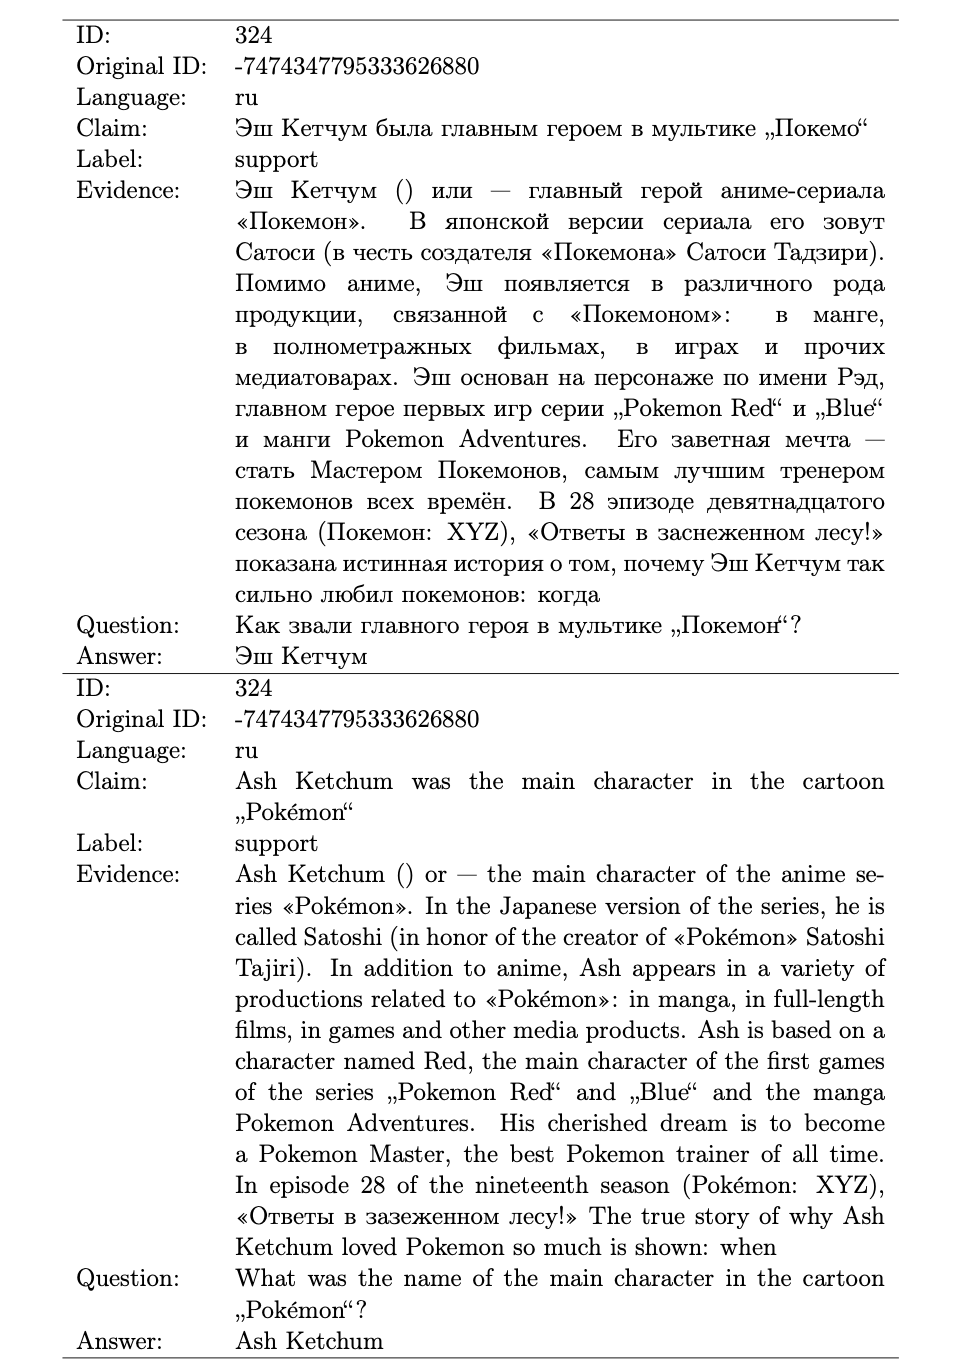
\includegraphics[scale=0.38]{figures/dataset.png}
    \caption{Example of one sample from the dataset. The second sample is the same, translated into English for the reader.}
    \label{fig:dataset}
\end{figure}

% \begin{table}[H]
%     \centering
%     \begin{tabular}{lp{10cm}}
%         \hline
%         ID: & 324 \\
%         Original ID: & -7474347795333626880 \\
%         Language: & ru \\
%         Claim: & Эш Кетчум была главным героем в мультике "Покемо" \\
%         Label: & support \\
%         Evidence: & Эш Кетчум () или — главный герой аниме-сериала «Покемон». В японской версии сериала его зовут Сатоси (в честь создателя «Покемона» Сатоси Тадзири). Помимо аниме, Эш появляется в различного рода продукции, связанной с «Покемоном»: в манге, в полнометражных фильмах, в играх и прочих медиатоварах. Эш основан на персонаже по имени Рэд, главном герое первых игр серии "Pokemon Red" и "Blue" и манги Pokemon Adventures. Его заветная мечта — стать Мастером Покемонов, самым лучшим тренером покемонов всех времён. В 28 эпизоде девятнадцатого сезона (Покемон: XYZ), «Ответы в заснеженном лесу!» показана истинная история о том, почему Эш Кетчум так сильно любил покемонов: когда \\
%         Question: & Как звали главного героя в мультике "Покемон"? \\
%         Answer: & Эш Кетчум \\
%         \hline
%         ID: & 324 \\
%         Original ID: & -7474347795333626880 \\
%         Language: & ru \\
%         Claim: & Ash Ketchum was the main character in the cartoon "Pokémon" \\
%         Label: & support \\
%         Evidence: & Ash Ketchum () or — the main character of the anime series «Pokémon». In the Japanese version of the series, he is called Satoshi (in honor of the creator of «Pokémon» Satoshi Tajiri). In addition to anime, Ash appears in a variety of productions related to «Pokémon»: in manga, in full-length films, in games and other media products. Ash is based on a character named Red, the main character of the first games of the series "Pokemon Red" and "Blue" and the manga Pokemon Adventures. His cherished dream is to become a Pokemon Master, the best Pokemon trainer of all time. In episode 28 of the nineteenth season (Pokémon: XYZ), «Ответы в зазеженном лесу!» The true story of why Ash Ketchum loved Pokemon so much is shown: when \\
%         Question: & What was the name of the main character in the cartoon "Pokémon"? \\
%         Answer: & Ash Ketchum \\
%         \hline
%     \end{tabular}
%     \caption{Example of one sample from the dataset. The second sample is the same, translated into English for the reader.}
%     \label{tab:dataset}
% \end{table}

The final datasets consists of 3 different sample types. The first is positive claim, that is matched with the evidence that supports the claim. Second type of sample is a negative claim, that is matched with the evidence that likely refutes the negative claim but containing the positive answer for the claim. To ensure the quality of the datasets and that the task were not that simple for the fact-checking model, the third type of samples were created in such a way that negative claim that is matched with the evidence containing the negative information based on which the claim was generated. The total number of the samples and its split is shown in the table~\ref{tab:dataset_stats}.

\begin{table}[h]
    \centering
    \begin{tabular}{l|l|ccccc}
        \hline
        Dataset & Type & Size & Support & Refute & $\text{Refute}^+$ & $\text{Refute}^-$ \\
        \hline
        \multirow{2}{*}{T5} & train & 47788 & 29751 & 18037 & 11784 & 6253 \\
        & dev & 2225 & 1145 & 1080 & 497 & 583 \\
        \multirow{2}{*}{mT5} & train & 47788 & 29751 & 18037 & 11784 & 6253 \\
        & dev & 2225 & 1145 & 1080 & 497 & 583 \\
        \hline
    \end{tabular}
    \caption{Overview of data file sizes. $\text{Refute}^+$ stands for negative claims matched with the evidence that contains correct answer. $\text{Refute}^-$ stands for negative claims matched with the evidence that supports incorrect answer.}
    \label{tab:dataset_stats}
\end{table}

% ################################################################################################################################################################################
% ################################################################################################################################################################################

\chapter{Experimental setup}\label{c6}
In this work Python was selected as the main programming language since it is popular in the machine learning community and contains many machine learning libraries that are used in this work. The vast majority of the code is based on the transformer library with a large collection of pre-trained models running on Pytorch~\cite{pytorch} backend.

\section{Top-K accuracy}
Top-k accuracy is a common evaluation metric used in retrieval tasks. It is used to measure the performance of a model in retrieving the most relevant documents or passages for a given query.

Top-K accuracy is calculated as the percentage of queries for which the model was able to retrieve at least one of the top k most relevant documents or passages. The value of k is typically set to a small number to ensure that the model is able to retrieve the most relevant documents or passages (i.e., k=100 in this work).

The basic equation for calculating top-k accuracy is as follows:
\begin{equation}
    \text{Top-k Accuracy} = \frac{\substack{Number\ of\ queries\ with\ at\ least\ one\\ relevant\ document\ in\ top\text{-}K\ ranked\ documents}}{Total\ number\ of\ queries}
\end{equation}
Top-k accuracy is a useful evaluation metric because it focuses on the ability of the model to retrieve the most relevant documents or passages for a given query. It is particularly useful for tasks where it is important to retrieve a small number of highly relevant documents or passages, such as in question answering task. Thus it is a valuable tool for measuring the performance of models in retrieving any relevant documents or passages for a given query.

% ################################################################################################################################################################################

\section{F-score}
F-score~\cite{f-score} describes model performance using a scale from zero to one. F-score itself is derived from two summary measures: precision and recall. Precision describes the proportion of entities which a model returns that are correct. Recall describes the proportion of all entities that potentially should be found, that a given model actually returns.

\subsection*{Precision and recall}
Precision measures the proportion of true positive results among the total number of positive results predicted by a model shown in equation~\ref{precision}. In other words, it is the ratio of true positives to the sum of true positives and false positives. High precision means that a model is producing few false positives relative to the number of true positives, indicating a low rate of false positives. However, precision alone may not give a complete picture of a model's performance, and it is often used in conjunction with the recall to provide a more comprehensive evaluation.

\begin{equation}
    P = \frac{|true~positives|}{|true~positives| + |false~positives|}\label{precision}
\end{equation}

Recall is a measure of a system's ability to identify all relevant instances of a target concept within a dataset. It is defined as the ratio of true positive results to the sum of true positive and false negative results shown in equation~\ref{recall}. In other words, recall measures the proportion of relevant items in the dataset that were correctly identified by the model. A high recall value indicates that the system is effective at finding all relevant instances of the target concept, while a low recall value indicates that many relevant instances were missed.

\begin{equation}
    R = \frac{|true~positives|}{|true~positives| + |false~negatives|}\label{recall}
\end{equation}

\subsection*{F1 score}
These metrics can be balanced out together. It is noted that these extreme situations, which were previously exploited, contrast with each other: when everything is returned, only a baseline precision is achieved, and returning just one thing typically results in a very low recall measure. Thus, it is a common practice to combine precision and recall with a weighted harmonic mean, known as an F-score:

\begin{equation}
    F_\beta = (1 + \beta^2)\frac{PR}{\beta^2P + R}
\end{equation}

The balance between precision and recall is determined by the coefficient $\beta$ in this equation, with high values favoring recall. A harmonic weighted mean of precision and recall is obtained in this manner. Typically F-score is used with $\beta$ = 1, c.f. its sometimes being called ``F1 score''.

\section{Rouge}
The quality of a summary is determined automatically by comparing it to other (ideal) summaries created by humans, using measures included in ROUGE (Recall-Oriented Understudy for Gisting Evaluation)~\cite{rouge}. The number of overlapping units such as n-gram, word sequences, and word pairs are counted between the computer-generated summary to be evaluated and the ideal summaries created by humans. In this work the measures \texttt{Rouge-N} and \texttt{Rouge-L} were used.

\subsection*{Rouge-N: N-gram co-occurrence statistics}
ROUGE-N is an n-gram recall between a candidate summary and a set of reference summaries. Rouge-N is computed as follows:
\begin{equation}
    ROUGE\text{-}N = \frac{\sum\limits_{S \in \{Summary\}} \sum\limits_{gram_n \in S} Count_{match}(gram_n)}{\sum\limits_{S \in \{Summary\}} \sum\limits_{gram_n \in S} Count(gram_n)}
\end{equation}
where $n$ stands for the length of the n-gram, $gram_n$, and $Count_{match}(gram_n)$ is the maximum number of n-grams co-occurring in a candidate summary and a set of reference summaries ($Summary$).

When multiple references are used, pairwise summary-level Rouge-N is computed between a candidate summary $s$ and every reference, $r_i$, in the reference set. The maximum of pairwise summary-level ROUGE-N scores is then taken as the final multiple reference Rouge-N score. This can be written as follows:
\begin{equation}
    ROUGE\text{-}N_{multi} = \text{argmax}_i ROUGE\text{-}N(r_i,s) 
\end{equation}
This procedure is also applied to computation of Rouge-L.
\subsection*{Rouge-L: longest common subsequence}
A sequence $Z = [z_1, z_2, ..., z_n]$ is a subsequence of another sequence $X = [x_1 , x_2 , ..., x_m ]$, if there exists a strict increasing sequence $[i_1, i_2, ..., i_k]$ of indices of $X$ such that for all $j=1,2,...,k$, we have $x_{ij}=z_j$~\cite{rouge_book}. When considering two sequences $X$ and $Y$, the common subsequence with maximum length is a longest common subsequence (LCS) that can be obtained.

To apply LCS in summarization evaulation, the summary sentence is viewed as a sequence of words. The intuition is that the longer the LCS of two summary sentences is, the more similar the two summaries are. In it was proposed to use LCS-based F-measure to estimate the similarity between two summaries $X$ of length $m$ and $Y$ of length $n$. $X$ stands for a reference summary sentence and $Y$ stands for candidate summary sentence, as follows: 
\begin{equation}
    R_{lcs} = \frac{LCS(X,Y)}{m}
\end{equation}

\begin{equation}
    P_{lcs} = \frac{LCS(X,Y)}{n}
\end{equation}

\begin{equation}
    F_{lcs} = \frac{(1 + \beta^2)R_{lcs}P_{lcs}}{R_{lcs}+\beta^2P_{lcs}}
\end{equation}
where $LCS(X,Y)$ is the length of a longest common subsequence of $X$ and $Y$, and $\beta = P_{lcs}/R_{lcs}$ when $?F_{lcs}/?R_{lcs} = ?F_{lcs}/?P_{lcs}$. $\beta$ is set to a very big number. Therefore, only $R_{lcs}$ is considered.

\section{Exact match score}\label{exact_match}
The exact match score is a metric used to evaluate the accuracy of natural language processing (NLP) models in predicting exact matches between two pieces of text.

In NLP tasks such as question-answering or text classification, the goal is often to predict a specific answer or label that exactly matches the true answer or label. The exact match score measures the percentage of predictions that are exactly correct, with no errors or variations from the true answer.

It is calculated as the number of exact matches between the predicted text and the true text, divided by the total number of examples:

\begin{equation}
   \text{EM} = \frac{\text{number of exact matches}}{\text{total number of examples}}.
\end{equation}

The exact match score is a useful metric for evaluating the performance of NLP models in scenarios where precision is more important than recall. It is more strict evaluation metric than other commonly used metrics, such as the F1 score, which may give partial credit for answers that are close but not exact.

\section{Implementation}
The implementation is divided into four main parts: mDPR, mGEN, T5 and translator. Each of these parts can be independent and thus none of the parts is explicitly dependent on the other. One of the main drawbacks is that each part requires different versions of the libraries, especially the pytroch and transformer libraries. These versions are described in the documentation for the code, which can be found on the github repository\footnote{\url{https://github.com/xkamen21/designing-a-multilingual-fact-checking-dataset-from-existing-question-answering-data.git}}. However, if the different parts of the code are run in the same order as described in chapter XX, the results will be the same as in this work.

\subsection{mDPR \& mGEN}
Since the implementations of multilingual dense passage retrieval and multilingual generator were already implemented in article~\cite{mDPR}, the code was taken from there. Some minor changes were applied in the code to eliminate some of the issues with the different versions of libraries. However, all the versions of libraries that were mention in the documentation of the code were used.

\subsection{T5}
Two implementations of the T5 model are presented in this work. Implementation for the T5 model was done with the own training loop and ``t5-base'' pre-trained model was used. However, there is nothing special about the implementation, as it was based on the HuggingFace\footnote{\url{https://huggingface.co}} tutorial. For the mT5 model the 'google/mt5-base' model was used from HuggingFace library. This implementation is based on library simpletransformers\footnote{\url{https://pypi.org/project/simpletransformers/0.26.0/}}, that consist of all the required functions for the training process. 

For the validation of the models two metrics was used namely rouge score (specificaly rouge-1, rouge-2 and rouge-L) and exact match score. The calculation of the rouges scores was done by the library evaluate library from HuggingFace. The implementation of the exact match score was taken from The Google AI Language Team\footnote{\url{https://github.com/google-research/language/blob/6019bb3ab669fff3a0bc65feb438caa58c262233/language/orqa/utils/eval_utils.py\#L97}}.


% ################################################################################################################################################################################
% ################################################################################################################################################################################

\chapter{Experiments}\label{c7}
The aim of this work was to compare two different approaches of creating fact-checking dataset from existing question-answering dataset. Several experiments were conducted to determine which of the approaches is better. As some stepts of dataset conversion are not easily evaluated automatically (such as translation evaluation and correctness of generated claims), this work resorted to Human Evaluation. To make the results as accurate as possible, most of the experiments consisted of human evaluation of the generated statements. The major part of the experiments consist of comparing the resulting datasets that were converted by the trained mT5 and T5 models. The Section~\ref{human_translation} deals with the evaluation of translation into other languages, as it turned out during the work~\ref{seq:languages_translation} that this part was the most critical for correct results.

For the claim validation 70 samples from each resulting dataset were randomly selected for experiments. These 70 samples were then given to 5 annotators who proceeded with the evaluation based on the attached instructions. The instructions can be seen in the~{\hypersetup{hidelinks}\nameref{apendix_a}}.

Human evaluation of the translations was performed only for the Russian language, as no sufficiently qualified persons were found for the other languages.
% \section{Human evaluation of translation} \label{human_translation}
\section{Translation} \label{human_translation}
The translation of datasets using machine learning proved to be one of the main challenges of the entire work. The work deals with diverse languages from several different language families. The languages contain also \emph{low-resource} languages (Bengali, Telugu). These language can have relatively small vocabulary, limited training data or they exhibit complex grammar, sentence structures, and rich morphology. This can lead to difficulties in training the translation model. Latin languages were translated well, but non-Latin languages were often translated into completely different statements, that are different from the original.

\subsection*{Human Evaluation}
One of the experiments was to perform a human evaluation of a machine translation into the Russian language. Evaluation was performed on 100 samples from the original XOR-TyDi QA dataset~\cite{xortydiqa}. One sample consisted of two parts. The first part contained Russian questions, which were then paired with English translations. The second part was the evaluation of the reverse translation from English to Russian. For this evaluation, English claim was taken and translated into Russian.

The translation was evaluated by an annotator who is a native speaker. The task of the annotator was to evaluate the translations into three different classes: \texttt{correct}, \texttt{incorrect} and \texttt{excellent}. The class \texttt{correct} stands for a translation that is correct with minor errors, the class \texttt{excellent} stands for a correct translation without any errors, and the class \texttt{incorrect} stands for a translation with important errors that affected the understanding of the sentence. The results can be seen in table~\ref{tab:ru_translation}.

\begin{table}[H]
    \centering
    \begin{tabular}{l|cccc}
        \hline
        Type & Samples & Good & Bad & Excellent \\
        \hline
        ru-en & 100 & 29\,\% & 26\,\% & 45\,\% \\
        en-ru & 100 & 18\,\% & 15\,\% & 67\,\% \\
        \hline
    \end{tabular}
    \caption{Russian evaluation of translations.}
    \label{tab:ru_translation}
\end{table}

As can be seen in the table, the results are very positive. The model can translate from Russian to English with more than 70\,\% success rate and from English to Russian with an success rate greater than 80\,\%. %accuracy

\subsection*{All Languages}\label{seq:languages_translation}
It is difficult to find annotators for each language that are native speakers. Therefore, the validation of the translation for other languages was done by translating an English sentence into the resulting language and then converting it back into English (back-translation). The task of this experiment was to check the translation of individual languages.

Data from the original FaVIQ dataset~\cite{faviq} were used for evaluation. Then 4 statements in the English language were taken from the dataset. These statements were then translated into all 7 languages and then translated back into the English language as you can see in Table~\ref{tab:all_translation}.

\begin{table}[H]
    \centering
    \begin{tabular}{l|p{11cm}}
        \hline
        Lang & Sequence \\
        \hline
        en & Additional information can be obtained. \\
        \hline
        ar & Additional information can be obtained. \\
        bn & You can receive more information. \\
        fi & Further information can be obtained. \\
        ja & You can get additional information. \\
        ko & You can get additional information. \\
        ru & For further information, please click here. \\
        te & More information is available. \\
        \hline
        \hline
        en & A sniper bullet hit Matt on the right side of the neck. \\
        \hline
        ar & Sniper bullet hit Matt on the right side of the neck. \\
        bn & A sniper went right on the right side of the car. \\
        fi & The sniper's bullet hit Matt on the right side of his neck. \\
        ja & The sniper's been shot on the right side of the mat. \\
        ko & The sniper bullet hit the mat on the right side of his neck. \\
        ru & A sniper bullet hit Matt on the right side of his neck. \\
        te & A snooze butt on the right side of the heat. \\
        \hline
        \hline
        en & He called his slave army the Black Guard. \\
        \hline
        ar & His slave army called his Black Guard. \\
        bn & He told his slave soldier in the Black Guard. \\
        fi & He called his slave army the Black Guard. \\
        ja & He called the Slaves Blackwords. \\
        ko & He called the slave army the Black Guard. \\
        ru & He called his army slaves a black guard. \\
        te & He was called the Black Guard of his servant’s army. \\
        \hline
        \hline
        en & Plants eventually formed chemical defenses against insects. \\
        \hline
        ar & Plants eventually formed chemical defences against insects. \\
        bn & Finally, the rains were prevented by Comprick. \\
        fi & The plants eventually formed chemical defenses against insects. \\
        ja & Finally, plants established a chemical protection against insects. \\
        ko & The plant eventually formed chemical defenses against insects. \\
        ru & Plants eventually created chemical protection against insects. \\
        te & In time, the fruitage produced by the family produced spiritual protection. \\
        \hline
    \end{tabular}
    \caption{Example of back translation.}
    \label{tab:all_translation}
\end{table}

The results have shown that the machine translation has a problem with languages like Bengali, Japanese or Telugu. Since the translation is part of the process of creating a dataset using the T5 model, the samples from these languages are of lower quality. It would be necessary to use another better model for translation. The other languages that are shown in table~\ref{tab:all_translation} were translated without major problems. It can be concluded that this methodology works well with Latine languages and could work with better models for other languages.

Additional manual analysis was performed on twenty samples based on back-translation. The results are shown in Table~\ref{tab:translation_procentage}.

\begin{table}[H]
    \centering
    \begin{tabular}{l|ccccccc}
        \hline
        Language & ar & bn & fi & ja & ko & ru & te \\
        Score & 65\,\% & 30\,\% & 75\,\% & 35\,\% & 70\,\% & 80\,\% & 25\,\% \\
        \hline
    \end{tabular}
    \caption{Results from manual back-translation evaluation over 20 samples.}
    \label{tab:translation_procentage}
\end{table}
As can be seen, the results showed that languages like Bengali, Japanese or Telugu were mistranslated more than 65\,\% of the time. On the other hand, using ``facebook/m2m100\_1.2B'' showed very good results in Korean. Thus, it can be considered that there are better models that could be used for machine translation in future works.

The evaluation of the next parts was based on usage of samples from the languages which translation was done correctly. This approach was selected because the goal of the work was not to evaluate the translation, but the resulting datasets.

\section{Human evaluation of claims}\label{sec:human_evaluation}
One of the main parts of the experiments was the human evaluation of the generated claims. The evaluation was performed by five annotators. They were provided 3-way annotation for 70 identical samples from both datasets (one generated by mT5 and the other generated by the T5 model). The annotator's task involved assessing the accuracy of the individual claims in terms of their generation. The factual side of the statement was not taken into account, and thus the annotators should have been purely concentrated on the claim conversion from the question-answer pairs. A/B testing was applied to evaluate the performance and effectiveness of the multilingual T5 model and monolingual T5 English model. The primary objective of A/B testing was to measure the performance of the models. By comparing the performance of the two models, statistical analysis was conducted to determine if there was a significant difference in performance between the models. The exact instructions which the annotators followed can be seen in {\hypersetup{hidelinks}\nameref{apendix_a}}.

The first part of the experiment was to assess whether the claim is generated correctly or incorrectly. In this evaluation, the annotators were not supposed to compare the claims with each other. They only evaluated the correctness of the generation. For a specific case where the statement was generated correctly but the information was not expressed explicitly, or the statement was interesting in some way to the annotator, he could mark the statement as interesting. This third class of evaluation is taken as correct but not entirely specific. The results of each annotator's evaluation are shown in Table~\ref{tab:anotators}.

\begin{table}[H]
    \centering
    \begin{tabular}{c|cccc}
         \hline
        Model & Annotator & Correct & Incorrect & Interesting \\
         \hline
        \multirow{5}{*}{T5} & 1 & 50 & 13 & 7 \\
         & 2 & 61 & 9 & 0 \\
         & 3 & 64 & 4 & 2 \\
         & 4 & 52 & 11 & 7 \\
         & 5 & 56 & 2 & 12 \\
         \hline
        \multirow{5}{*}{mT5} & 1 & 30 & 34 & 6 \\
         & 2 & 43 & 25 & 2 \\
         & 3 & 55 & 7 & 8 \\
         & 4 & 47 & 16 & 7 \\
         & 5 & 47 & 10 & 13 \\
         \hline
    \end{tabular}
    \caption{Results from annotators from 70 samples of the dataset.}
    \label{tab:anotators}
\end{table}

It can be seen from the results in Table~\ref{tab:anotators} that both models generated statements with very good accuracy. For a more reliable evaluation an objective score was calculated for each individual model. This score was derived from the number of correct results for each sample (the sum of interesting and correct statements), which was then divided by the number of annotators who participated in the evaluation. After all samples were calculated, the values were summed to obtain the final model score. For a perfect evaluation, the model had to score 70 points, which would mean that all annotators would rate all samples as correct or interesting.

% nejoptimistejsi a nepisimiestejsi (vsichni pro jeden pro)
% disclaimer biases

The next objective for the annotators was to select claim they would prefer as more accurately generated. Both evaluation ways results are shown in Table~\ref{tab:total_score}.

\begin{table}[H]
    \centering
    \begin{tabular}{l|cccc}
        \hline
        Model & Examples & Total Score & Score [\%] & Preference [\%] \\
        \hline
        T5 & \multirow{2}{*}{70} & 62 & 89 & 56 \\
        mT5 & & 51.4 & 73 & 27\\
        \hline
    \end{tabular}
    \caption{Results of custom metrics over results from annotators. The ``Preferences'' column contains only preferences from annotators for the model. The remaining 17\,\% were rated as cannot be judged.}
    \label{tab:total_score}
\end{table}


As can be seen, the results show that the T5 model resulted in better score. For T5 the annotators determined 89\,\% of the generated statements to be correct, compared to the mT5 model, which generated a resulting accuracy of 73\,\%. Thus, the preference of the generated statements prevailed for the T5 model, when out of the total 70 samples. The annotators were in favor of the T5 model.

The above metrics considered each individual response from the annotators. For a different point of view, table~\ref{tab:agreement} shows correctly identified statements using the methodology of \texttt{at least one agreement} and \texttt{unanimous agreement}.

\begin{table}[H]
    \centering
    \begin{tabular}{l|cccc}
        \hline
        Type & \multicolumn{2}{c}{mT5} & \multicolumn{2}{c}{T5} \\
         & Count & In precent & Count & In precent \\
        \hline
        at least one agreement & 66 & 94\,\% & 69 & 99\,\% \\
        unanimous agreement & 33 & 47\,\% & 49 & 70\,\% \\
        \hline
    \end{tabular}
    \caption{The table shows the number of samples for which the annotators agreed on the correct one "\texttt{unanimous agreement}" and the number of samples for which at least one annotator determined the sample to be correct "\texttt{at least one agreement}".}
    \label{tab:agreement}
\end{table}

Model preference was evaluated based on the majority of individual preferences. In the table~\ref{tab:total_score} we can see that 39 samples were preferred by the annotators for the T5 model and only 19 samples were preferred for the mT5 model. The remaining 12 samples could not be judged as they had an inconclusive preference. For a more accurate evaluation, individual preferences were converted into numbers. For the T5 model, the preference was converted to value of -1, for mT5 the preference was converted to value of 1, and the samples that could not be assessed were set to 0. These values were then added up. The result is shown in Figure~\ref{fig:model_results}.

\begin{figure}[H]
    \centering
    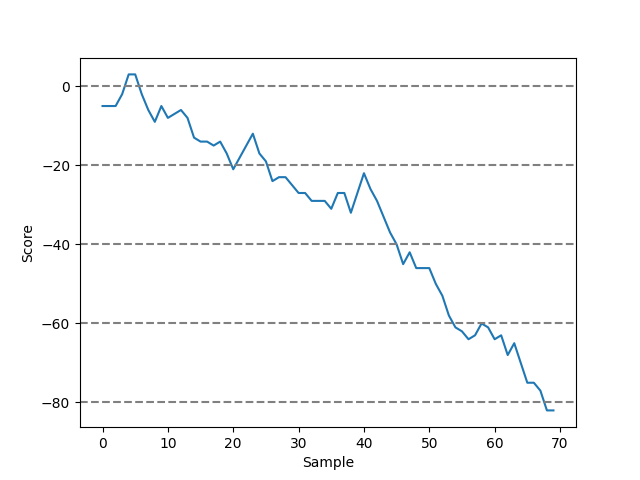
\includegraphics[scale=0.6]{figures/model_results.png}
    \caption{Result of custom metric for annotators preference.}
    \label{fig:model_results}
\end{figure}

As can be seen, most of the preferences were still leaning towards the T5 model, but the difference is no longer so significant. The maximum score that each model could get was 350 for mT5 and -350 for T5. The resulting score ended up at -82 in favor of the T5 model. 

Unfortunately, a disclaimer must be given here, as the data that was passed to the annotators contained information about which claim was generated by which model and therefore the annotators could be biased by previous results. Thus, this section should be re-examined and done without identifying models in future works.

However, the results of both models are very positive. If we take into account that the use of the T5 model requires additional computing power for translation and the generation process itself is then that much longer, then the use of the multilingual T5 model is definitely an interesting option.

\section{Discussion of the final dataset quality}
The translation of the text was worse than expected. Therefore, an optimistic and pessimistic estimate of the size of the usable dataset was made. The estimate is based on three baseline values that were evaluated during the experiments. The first value is the number of generated claims, which is described in Section~\ref{pos_neg_answers}. The second value is the success rate of text translation in individual languages, which was obtained using back translation in Section~\ref{human_translation}. These values are shown in Table~\ref{tab:dataset_quality}.

\begin{table}[H]
    \centering
    \begin{tabular}{l|lccccccc}
        \hline
        Language & & Ar & Bn & Fi & Ja & Ko & Ru & Te \\
        \hline
        \multirow{2}{*}{\# Samples} & Train & 17900 & 4108 & 8655 & 1891 & 2224 & 7909 & 5101 \\
         & Dev & 610 & 311 & 445 & 60 & 161 & 429 & 209 \\
        Translation & & 65\,\% & 30\,\% & 75\,\% & 35\,\% & 70\,\% & 80\,\% & 25\,\% \\
        \hline
    \end{tabular}
    \caption{Values for the estimation of the final datasets size.}
    \label{tab:dataset_quality}
\end{table}

The last value refers to the success rate of the claim generation itself using individual models. The claim generation value was used from two evaluation heuristics. Based on this estimate, an estimate of the size of the useful data in the dataset was then evaluated.

The first heuristic was calculated using an optimistic evaluation, where the success rate value of the claim generation was obtained by the \texttt{at least one agreement} method~\ref{sec:human_evaluation}. In this case, the monolingual T5 model had a success rate of 99\,\% and the multilingual mT5 model had a success rate of 94\,\%. For each language, the number of successfully translated samples was calculated in the way that number of samples from each language were miltyplied with the success rate of the translation for the target language. For Arabic, the value of correctly translated samples was calculated: $0.65 * 17900 = 11635$ for the training dataset and $0.65 * 610 = 396$ for the validation dataset. The estimation is that 11635 samples in the training data set and 396 samples in the validation data set were correctly translated. This methodology was performed for all languages.

As a result of multiplying the correctly translated samples with the success of generating an individual model, the value of the number of usable samples in each data set was reached. Thus, for the values calculated for Arabic and the T5 model, the resulting number of usable samples would be calculated: $11635 * 0.99 = 11518$ for the training dataset. This was done for a single model in particular over all languages. The resulting count shows how many usable causes from each language a single data set contains.

The second heuristic was calculated using an pessimistic evaluation, where the success rate value of the claim generation was obtained by the \texttt{unanimous agreement} method~\ref{sec:human_evaluation}. The same methodology was used as for the first estimation. The values of the success rate were 70\,\% for the T5 model and 47\,\% for the mT5 model. The final results of the datasets are shown in table~\ref{tab:result_data_size}.

% 0.65 Ar
% 0.30 Bn
% 0.75 Fi
% 0.35 Ja
% 0.70 Ko
% 0.80 Ru
% 0.25 Te

% T5
% 0.99 Opt
% 0.70 Pes

% mT5
% 0.96 Opt
% 0.47 Pes

\begin{table}[H]
    \centering
    \begin{tabular}{l|l|lccccccc|c}
        \hline
        Model & Variant & Dataset & Ar & Bn & Fi & Ja & Ko & Ru & Te & Total \\
        \hline
        \multirow{4}{*}{T5} & \multirow{2}{*}{Opt} & Train & 11518 & 1220 & 6426 & 655 & 1541 & 6264 & 1262 & \textbf{28887} \\
         & & Dev  & 393 & 92 & 330 & 21 & 112 & 340 & 52 & \textbf{1340}\\
         \cline{3-11}
         & \multirow{2}{*}{Pess} & Train  & 8144 & 863 & 4544 & 463 & 1090 & 4429 & 893 & \textbf{20426} \\
         & & Dev  & 278 & 65 & 234 & 15 & 79 & 240 & 37 & \textbf{948}\\
        \hline
        \multirow{4}{*}{mT5} & \multirow{2}{*}{Opt} & Train & 11169 & 1183 & 6232 & 635 & 1495 & 6074 & 1224 & \textbf{28013} \\
         & & Dev  & 381 & 90 & 320 & 20 & 108 & 329 & 50 & \textbf{1298}\\
         \cline{3-11}
         & \multirow{2}{*}{Pess} & Train & 5468 & 579 & 3051 & 311 & 732 & 2974 & 599 & \textbf{13714} \\
         & & Dev  & 186 & 44 & 157 & 10 & 53 & 161 & 25 & \textbf{636}\\
        \hline
    \end{tabular}
    \caption{The estimation number of final samples in each data set. The ``Variant'' column represents optimistic and pessimistic heuristics.}
    \label{tab:result_data_size}
\end{table}

It can be seen from the results that the converted datasets still have a large number of samples. However, some languages have a smaller number of samples, almost unusable. This is due to poor machine translation where a large number of samples were mistranslated. The heuristics used this fact into account. Heuristics themselves have their limitations. This is because random samples were not selected to evaluate the correct generation of claims. Instead, samples that made sense when translated were used. One sample means the translated question, answer, and claim itself from the target dataset. This may have filtered out samples from low-resource languages and thus cannot guarantee that the models generate claims with the same accuracy for these languages as well.

Nevertheless, using a better translation model for low-resource languages could make the evaluations more accurate. The results could then be more balanced for all languages. Therefore, the translation turned out to be the main critical point of this work. The conversions of claims themselves turned out to be almost perfect. And so the work shows beneficial information that could be used to convert an existing question-answering dataset into a fact-checking dataset.

\section{Fact-checking using TF-IDF}\label{seq:experiments_tfidf}
In this section, the machine evaluation of resulting dataset was performed with help of logistic regression classifier to determine if a claim is supported or refuted.

Logistic regression is a commonly used classification algorithm that is well suited for binary classification tasks. It works by estimating the probability that an input belongs to a particular class based on the values of its features. The model uses a logistic function to map the input features to the output probabilities.

In the evaluation phase, the logistic regression model was trained on the training data and then used to make predictions on the validation data. The confusion matrix~\ref{fig:mt5_regression} was used to evaluate the performance of the models in terms of true positives, true negatives, false positives, and false negatives. The result for the mT5 model is shown in table~\ref{tab:mT5_classification_report}.

\begin{figure}[H]
    \centering
    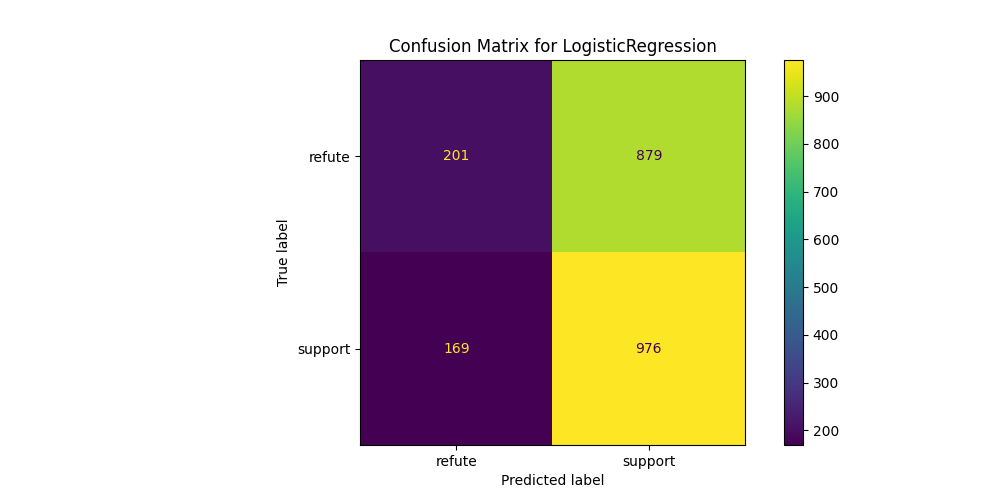
\includegraphics[scale=0.5]{figures/mt5_LogisticRegression.png}
    \caption{mt5 logistic regression}
    \label{fig:mt5_regression}
\end{figure}

\begin{table}[H]
    \centering
    \begin{tabular}{l|ccccc}
        \hline
        & Precision & Recall & F1-score & \# Samples & Accuracy \\
        \hline
        refute & 0.54 & 0.19 & 0.28 & 1080 & \multirow{2}{*}{0.53} \\
        support & 0.53 & 0.85 & 0.65 & 1145 &  \\
        \hline
    \end{tabular}
    \caption{Classification report for dataset from mT5 model.}
    \label{tab:mT5_classification_report}
\end{table}

% Precision is the fraction of true positives among all predicted positives. For the "refute" class, it means that out of all the claims predicted as "refute", 54\,\% of them are actually "refute". For the "support" class, it means that out of all the claims predicted as "support", 53\,\% of them are actually "support".

% Recall is the fraction of true positives among all actual positives. For the "refute" class, it means that out of all the "refute" claims, 19\,\% of them are correctly identified as "refute" by the model. For the "support" class, it means that out of all the "support" claims, 85\,\% of them are correctly identified as "support" by the model.

% F1-score is the harmonic mean of precision and recall. It balances both precision and recall and is a better measure of overall model performance. For the "refute" class, the F1-score is 0.28, while for the "support" class it is 0.65.

The classification report shows that the model is better at predicting the "support" class compared to the "refute" class. The model has a high precision for both classes, but the recall for "refute" class is low. This means that the model is not able to correctly identify all "refute" claims, and is more biased towards predicting "support" claims.

After evaluating the T5 model on the same dataset, it was found that the confusion matrix~\ref{fig:t5_regression} and classification report~\ref{tab:T5_classification_report} were almost identical to the T5 model.

\begin{figure}[H]
    \centering
    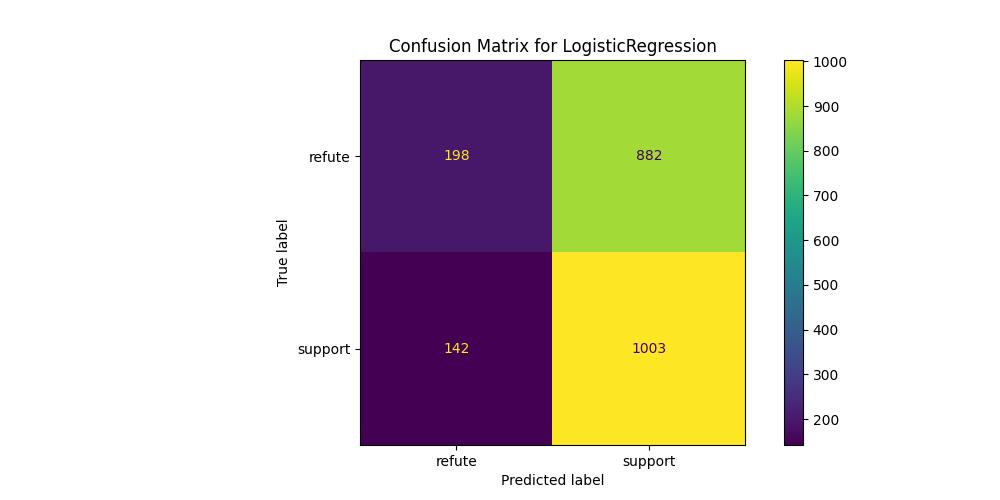
\includegraphics[scale=0.5]{figures/t5_LogisticRegression.png}
    \caption{T5 logistic regression}
    \label{fig:t5_regression}
\end{figure}

\begin{table}[H]
    \centering
    \begin{tabular}{l|ccccc}
        \hline
        & Precision & Recall & F1-score & \# Samples & Accuracy \\
        \hline
        refute & 0.58 & 0.18 & 0.28 & 1080 & \multirow{2}{*}{0.54}\\
        support & 0.53 & 0.88 & 0.66 & 1145 & \\
        \hline
    \end{tabular}
    \caption{Classification report for dataset from T5 model.}
    \label{tab:T5_classification_report}
\end{table}

% Based on the Cohen's kappa value of \textbf{0.04} for mT5 model dataset and value of \textbf{0.06} for T5 model dataset obtained from the predicted labels by the logistic regression model and the true labels, it appears that the dataset is challenging for the model. A Cohen's kappa value of 0 indicates complete randomness, while a value of 1 indicates perfect agreement between predicted and true labels.
These results suggest that the performance of the T5 model is similar to the mT5 model in classifying claims as either supported or refuted. This finding showed that there is almost no difference for machine classification between the two datasets. The classification model was able to correctly predict supported claims on both datasets, but failed to correctly identify refuted claims.

The resulting classification report for all languages from each dataset can be seen in Table~\ref{tab:all_classification_report}.

\begin{table}[H]
    \centering
    \begin{tabular}{l|llccccc}
        \hline
        Dataset & Lang &  & Precision & Recall & F1-score & \# Samples & Accuracy \\
        \hline
        \multirow{14}{*}{T5} & \multirow{2}{*}{Ar} & refute & 0.55 & 0.13 & 0.21 & 291 & \multirow{2}{*}{0.53} \\
         & & support & 0.53 & 0.90 & 0.67 & 319 &  \\
        \cline{2-8}
         & \multirow{2}{*}{Bn} & refute & 0.59 & 0.46 & 0.52 & 170 & \multirow{2}{*}{0.53} \\
         & & support & 0.48 & 0.60 & 0.54 & 141 &  \\
        \cline{2-8}
         & \multirow{2}{*}{Fi} & refute & 0.56 & 0.11 & 0.18 & 199 & \multirow{2}{*}{0.56} \\
         & & support & 0.56 & 0.93 & 0.70 & 246 &  \\
        \cline{2-8}
         & \multirow{2}{*}{Ja} & refute & 0.50 & 0.04 & 0.07 & 25 & \multirow{2}{*}{0.58} \\
         & & support & 0.59 & 0.97 & 0.73 & 35 &  \\
        \cline{2-8}
         & \multirow{2}{*}{Ko} & refute & 0.49 & 0.26 & 0.34 & 68 & \multirow{2}{*}{0.57} \\
         & & support & 0.60 & 0.80 & 0.68 & 93 &  \\
        \cline{2-8}
         & \multirow{2}{*}{Ru} & refute & 0.61 & 0.16 & 0.25 & 226 & \multirow{2}{*}{0.50} \\
         & & support & 0.49 & 0.89 & 0.63 & 203 &  \\
        \cline{2-8}
         & \multirow{2}{*}{Te} & refute & 0.73 & 0.11 & 0.19 & 101 & \multirow{2}{*}{0.55} \\
         & & support & 0.54 & 0.96 & 0.69 & 108 &  \\
        \hline
        \hline
        \multirow{14}{*}{mT5} & \multirow{2}{*}{Ar} & refute & 0.52 & 0.16 & 0.24 & 291 & \multirow{2}{*}{0.53} \\
         & & support & 0.53 & 0.87 & 0.66 & 319 &  \\
        \cline{2-8}
         & \multirow{2}{*}{Bn} & refute & 0.58 & 0.45 & 0.50 & 170 & \multirow{2}{*}{0.52} \\
         & & support & 0.47 & 0.60 & 0.53 & 141 &  \\
        \cline{2-8}
         & \multirow{2}{*}{Fi} & refute & 0.48 & 0.08 & 0.14 & 199 & \multirow{2}{*}{0.55} \\
         & & support & 0.56 & 0.93 & 0.70 & 246 &  \\
        \cline{2-8}
         & \multirow{2}{*}{Ja} & refute & 0.00 & 0.00 & 0.00 & 25 & \multirow{2}{*}{0.55} \\
         & & support & 0.57 & 0.94 & 0.71 & 35 &  \\
        \cline{2-8}
         & \multirow{2}{*}{Ko} & refute & 0.45 & 0.29 & 0.36 & 68 & \multirow{2}{*}{0.55} \\
         & & support & 0.59 & 0.74 & 0.66 & 93 &  \\
        \cline{2-8}
         & \multirow{2}{*}{Ru} & refute & 0.59 & 0.19 & 0.29 & 226 & \multirow{2}{*}{0.50} \\
         & & support & 0.49 & 0.85 & 0.62 & 203 &  \\
        \cline{2-8}
         & \multirow{2}{*}{Te} & refute & 0.44 & 0.07 & 0.12 & 101 & \multirow{2}{*}{0.51} \\
         & & support & 0.51 & 0.92 & 0.66 & 108 &  \\
        \hline
    \end{tabular}
    \caption{Classification report for all languages from both datasets.}
    \label{tab:all_classification_report}
\end{table}

% ################################################################################################################################################################################

% ################################################################################################################################################################################

\chapter{Conclusion}\label{c8}
The objective of this work was to propose, develop and compare different approaches to converting a multilingual fact-checking dataset from existing question-answering (QA) dataset. The dataset was converted from an existing XOR-TyDi QA dataset. From this dataset, question-answer-passage triplets were constructed in 7 diverse languages from which claims were generated. The proposed systems are based on generative transformer model T5. Two main approaches were tested. The first was to adapt the English monolingual model to a multilingual task using machine translation to translate both input and output. The second approach was to use a natively multilingual model that would take input in any language and generate statements directly in the target language.

In order to create a system for automatic data set conversion, it was necessary to become familiar with the current problems of multilingual fact-checking and the importance of using sources from different languages. Therefore, the work describes the relevant data sources that were needed to convert the datasets. The work also examines an already existing approach for converting datasets. The work is based on this approach.

The answers were generated using the adopted CORA system. An evidence (passage) was added, resulting in a question-answer-passage triplet. These triplets were translated into the English and passed to the T5 model. The model converted question-answer pairs presented in triplet into the resulting claims in English. Each claim was then translated back to the target language. The second approach was based on mT5 model that takes the triplets in the original languages. The mT5 converted the question-answer pair presented in the triplet into the claim. The converted claims were already in the target language without help of translation. Datasets were then created based on the generated claims.

To analyze possible biases label specific claim biases, the logistic-regression based TF-IDF classifier was trained. The classifier achieved accuracy close to  0.5 for both converted datasets. The qualitative value of the dataset was evaluated by several annotators with positive results compare to the FaVIQ where they achieved success rate of 95\,\%. The claims generated from multilingual model achieved a success rate of 73\,\% compared to monolingual model with a success rate of 88\,\%. However, compared to the FaVIQ, only the smaller model variants of the T5 models were used. 

The result of this work is that the conversion of a multilingual dataset from an existing QA dataset is possible, but with the use of more complex models both for translation and for generating the resulting claims, it would be possible to achieve much better results. The \emph{low-resource} languages were translated with the success rate around 35\,\%.
  \else
    \input{projekt-01-kapitoly-chapters}
  \fi
  
  % Kompilace po částech (viz výše, nutno odkomentovat a zakomentovat input výše)
  % Compilation piecewise (see above, it is necessary to uncomment it and comment out input above)
  %\subfile{chapters/projekt-01-uvod-introduction}
  % ...
  %\subfile{chapters/projekt-05-zaver-conclusion}

  % Pouzita literatura / Bibliography
  % ----------------------------------------------
\ifslovak
  \makeatletter
  \def\@openbib@code{\addcontentsline{toc}{chapter}{Literatúra}}
  \makeatother
  \bibliographystyle{bib-styles/Pysny/skplain}
\else
  \ifczech
    \makeatletter
    \def\@openbib@code{\addcontentsline{toc}{chapter}{Literatura}}
    \makeatother
    \bibliographystyle{bib-styles/Pysny/czplain}
  \else 
    \makeatletter
    \def\@openbib@code{\addcontentsline{toc}{chapter}{Bibliography}}
    \makeatother
    \bibliographystyle{bib-styles/Pysny/enplain}
  %  \bibliographystyle{alpha}
  \fi
\fi
  \begin{flushleft}
  \bibliography{project-20-bibliography}
  \end{flushleft}

  % vynechani stranky v oboustrannem rezimu
  % Skip the page in the two-sided mode
  \iftwoside
    \cleardoublepage
  \fi

  % Prilohy / Appendices
  % ---------------------------------------------
  \appendix
\ifczech
  \renewcommand{\appendixpagename}{Přílohy}
  \renewcommand{\appendixtocname}{Přílohy}
  \renewcommand{\appendixname}{Příloha}
\fi
\ifslovak
  \renewcommand{\appendixpagename}{Prílohy}
  \renewcommand{\appendixtocname}{Prílohy}
  \renewcommand{\appendixname}{Príloha}
\fi
%  \appendixpage

% vynechani stranky v oboustrannem rezimu
% Skip the page in the two-sided mode
%\iftwoside
%  \cleardoublepage
%\fi
  
\ifslovak
%  \section*{Zoznam príloh}
%  \addcontentsline{toc}{section}{Zoznam príloh}
\else
  \ifczech
%    \section*{Seznam příloh}
%    \addcontentsline{toc}{section}{Seznam příloh}
  \else
%    \section*{List of Appendices}
%    \addcontentsline{toc}{section}{List of Appendices}
  \fi
\fi
  \startcontents[chapters]
  \setlength{\parskip}{0pt} 
  % seznam příloh / list of appendices
  % \printcontents[chapters]{l}{0}{\setcounter{tocdepth}{2}}
  
  \ifODSAZ
    \setlength{\parskip}{0.5\bigskipamount}
  \else
    \setlength{\parskip}{0pt}
  \fi
  
  % vynechani stranky v oboustrannem rezimu
  \iftwoside
    \cleardoublepage
  \fi
  
  % Přílohy / Appendices
  \ifenglish
    \newpage
\section*{Appendix A} \label{apendix_a}

\subsection*{Introduction into the task}
The aim of my thesis is to evaluate two different approaches to building a multilingual dataset for fact-checking models.
What does a fact-checking model mean? In simple terms, you can imagine that a fact is passed to the model, for example: ''\textit{President Barack Obama was born in 2012.}`` and the model tries to evaluate whether that fact is \texttt{true} or \texttt{false}. To train such a model, it is important to have a dataset that contains as many examples as possible. Each example must contain a claim, an evidence, that supports or refutes the claim and the correct label (in my case: \texttt{refute}/\texttt{support}). Nowadays, there are already many datasets, but they are all mostly only in English and thus there is a lack of multilingual datasets.

A similar task is a model that answers questions. A question is passed to the model and the model generates an answer. To train such a model, one needs a dataset that contains the question-answer pair, ideally including a record of where the answer to the question occurred.

It can be seen that the approach to training the two models is quite similar. Therefore, I decided to create the fact-checking dataset from another existing multilingual dataset for the question-answering model that contains question-answer pairs. From these pairs, the seq2seq model (a model that has a sequence of words as input and the output is again a sequence of words) was trained to generate a fact, since in the question we have information about what the answer specifically refers to, and the answer itself is the information we want to transfer to the fact.
\begin{table}[h]
    \centering
    \begin{tabular}{cc}
     \textbf{Question}: When was Barack Obama born? & \textbf{Answer}: 1961 \\
    \end{tabular}
    \caption{Example of the Question-Answer pair.}
\end{table}

Since generating a fact is not a trivial task for the model (especially for multilingual data), two different approaches were therefore taken. 
\begin{itemize}
    \item The first approach is to train the model on the English dataset. The translated input (question and answer) is then passed to the model. The model returns the output (fact) in English, which is then translated back into the original language.
    \item  The second approach is to train a multilingual model that receives the input in the desired language and therefore returns the output in the desired language.

\end{itemize}

\subsection*{Task for annotators}
Automatic evaluation of the results of each approach is difficult to perform and therefore human evaluation is also important. In the attached file you have received an excel that contains the generated claim (translated into the english) from both models. These results need to be manually analyzed to determine whether the resulting fact is understandable or not.

Therefore, I would like to ask you to perform a manual analysis. One line of the file corresponds to one example from the dataset. Each line contains information about the original question and its answer. This is followed by the claim that was generated by model A and then the claim that was generated by model B. Your task is to assign to each claim one of your answers at your discretion: whether the claim is correct, whether the claim is wrong, or whether the claim is generated in an interesting way. An interesting claim contains all the necessary information, but is not quite as specific as you would expect.

\begin{table}[h]
    \centering
    \begin{tabular}{c}
        \textbf{Question}: Where was Barack Obama born? \textbf{Answer}: USA\\
        \textbf{Claim}: Barack Obama was born in Honolulu, Hawaii
    \end{tabular}
    \caption{Example of the generated calim from the Question-Answer pair.}
\end{table}

\subsubsection*{ToDo list for annotators}
In summary, you need to add a label to each claim and then select a preference for the claim that you think is better generated:

\begin{enumerate}
    \item fill in the column to the right of the claim with one of the answers:
    \begin{table}[h]
        \centering
        \begin{tabular}{|c|c|c|}
            \hline
            correct & incorrect & interesting \\
            \hline
        \end{tabular}
    \caption{Labels for the claim validation.}
    \end{table}
    \item fill in the last column with your preference for the generated fact based on the model as follows:
    \begin{table}[h]
        \centering
        \begin{tabular}{|c|c|c|}
            \hline
            A & B & CBJ \\
            \hline
        \end{tabular}
    \caption{Labels for the claim preference.}
    \end{table}
\end{enumerate}
\noindent * (CBJ stands for: cannot be judged)
  \else
    \input{projekt-30-prilohy-appendices}
  \fi
  
  % Kompilace po částech (viz výše, nutno odkomentovat)
  % Compilation piecewise (see above, it is necessary to uncomment it)
  %\subfile{projekt-30-prilohy-appendices}
  
\end{document}
